%\cleardoublepage

\chapter{EXPERIMENTAL RESULTS AND UNCERTAINTY}
\label{ch:ExpResult}

\section{Data Analysis}
\label{sec:ExpResult:HeatRej:DataAnalysis}
	
The heat rejection and heat extraction data were analyzed by treating the water on the outside of the heat exchanger as having an infinite capacity. Then, the $\varepsilon$--NTU method was used to determine the heat exchanger's overall heat transfer coefficient. From this, the outside convection heat transfer coefficient could then be backed out given that the values for the remaining thermal resistance components can be accurately estimated or otherwise determined.

SWHE heat transfer rate was calculated by Equation \ref{eq:ExpResult:HeatRej:DataAnalysis:HXHeatRate} from the circulating fluid mass flow rate along with entering and exiting fluid temperatures. The maximum possible heat transfer rate is given by Equation \ref{eq:ExpResult:HeatRej:DataAnalysis:HXMaxHeatRate}.  Surface water temperature is measured as described in Sections \ref{subsec:ExpMethod:HeatRej:Apparatus} and \ref{subsec:ExpMethod:HeatExtr:Apparatus}; the value was calculated as a weighted average of the three measurements as given in Equation \ref{eq:ExpMethod:HeatRej:Apparatus:PondTemp}. Circulating fluid mass flow rate is calculated from Equation \ref{eq:ExpResult:HeatRej:DataAnalysis:mDot} from the volumetric flow rate measured by the flow meter and the circulating fluid density.

	\begin{equation}
		\dot{Q}_{SWHE} = \dot{m}_f \, c_{p,f} \, (T_{f,in}-T_{f,out})
		\label{eq:ExpResult:HeatRej:DataAnalysis:HXHeatRate}
	\end{equation}
	

	\begin{equation}
		\dot{Q}_{max}=\dot{m}_f \, c_{p,f} \, (T_{f,in}-T_{sw})
		\label{eq:ExpResult:HeatRej:DataAnalysis:HXMaxHeatRate}
	\end{equation}
	
	\begin{equation}
		\dot{m} = \dot{V} \cdot \rho_f
		\label{eq:ExpResult:HeatRej:DataAnalysis:mDot}
	\end{equation}
	
Heat exchanger effectiveness is calculated with Equation \ref{eq:ExpResult:HeatRej:DataAnalysis:HXEffectivness}. Then, the heat exchanger overall heat transfer coefficient $U A_s$ is determined with Equations \ref{eq:ExpResult:HeatRej:DataAnalysis:HXntu} and \ref{eq:ExpResult:HeatRej:DataAnalysis:HXua}. Equation \ref{eq:ExpResult:HeatRej:DataAnalysis:HXntu} is used in heat exchanger analysis for situations when one side of the heat exchanger is considered to have an infinite capacity. For our case, the surface water temperature is not expected to change temperature due to the heat rejected or extracted by the SWHE. This is because we expect the mass, and thus, thermal capacitance of the surface water to be very large when compared to the heating or cooling load. Because we don't expect the surface water temperature to be notably affected by the SWHE, Equation \ref{eq:ExpResult:HeatRej:DataAnalysis:HXntu} is valid.

	\begin{equation}
		\varepsilon=\frac{\dot{Q}_{SWHE}}{\dot{Q}_{max}}
		\label{eq:ExpResult:HeatRej:DataAnalysis:HXEffectivness}
	\end{equation}
	
	\begin{equation}
		\mbox{NTU} = - \ln \, (1-\varepsilon)
		\label{eq:ExpResult:HeatRej:DataAnalysis:HXntu}
	\end{equation}
	
	\begin{equation}
		UA_s=\mbox{NTU} \, \dot{m}_f \, c_{p,f}
		\label{eq:ExpResult:HeatRej:DataAnalysis:HXua}
	\end{equation}
	
From the heat exchanger overall heat transfer coefficient, the total thermal resistance of the heat exchanger can be determined by Equation \ref{eq:ExpResult:HeatRej:DataAnalysis:HXrTotal}. At this point, the outside convective resistance can be determined, given that the inside convective resistance and pipe wall conductive resistance values can be calculated independently.

	\begin{equation}
		(UA_s)^{-1}=R_{tot}=R_{conv,i}+R_{cond}+R_{conv,o}
		\label{eq:ExpResult:HeatRej:DataAnalysis:HXrTotal}
	\end{equation}
	
To calculate the inside thermal resistance, the inside Nusselt number as correlation developed by \cite{RogersMayhew1964} is used. This correlation for Nusselt number (Equation \ref{eq:ExpResult:HeatRej:DataAnalysis:RogersNusseltNo}) given by \cite{RogersMayhew1964} is a heat transfer correlation for helically coiled tubes under isothermal exterior tube surface conditions. Included in the correlation is the ratio of pipe inside diameter to coil diameter which helps quantify the increase in heat transfer due to the secondary flows that occur in helically coiled pipes. \cite{RogersMayhew1964}, \cite{SebanMclaughlin1963}, as well as others, have noted that secondary flows induced in helical pipes due to the centrifugal forces associated with the flow and curvature cause increases in heat transfer rate. Because of these secondary flows, a straight pipe approximation is insufficient and the \cite{RogersMayhew1964} correlation was selected as the best approximation for inside Nusselt number. The mean coil diameter is calculated by averaging the SWHE inside and outside diameters as is indicated in Equation \ref{eq:ExpResult:HeatRej:DataAnalysis:AveCoilDia}. Coil inside and outside diameters can been seen in Figure \ref{fig:Intro:HXOverview:SpHelHX:SWHESchematic}.

	\begin{equation}
		\mbox{Nu}_{D,i}=0.023 \, Re_{D_{i,p}}^{0.85} \, Pr^{0.4} \, \left(\frac{D_{i,p}}{D_{ave,SWHE}}\right)^{0.1}
		\label{eq:ExpResult:HeatRej:DataAnalysis:RogersNusseltNo}
	\end{equation}
	
	\begin{equation}
		D_{ave,SWHE} = \frac{D_{i,SWHE} + D_{o,SWHE}}{2}
		\label{eq:ExpResult:HeatRej:DataAnalysis:AveCoilDia}
	\end{equation}

Coil inside convection coefficient and inside convective thermal resistance are calculated directly from Equations \ref{eq:ExpResult:HeatRej:DataAnalysis:InsideConvCoeff} and \ref{eq:ExpResult:HeatRej:DataAnalysis:InsideConvResist}.
	
	\begin{equation}
		h_{conv,i}=\frac{Nu_{D,i} \, k_f}{D_{p,i}}
		\label{eq:ExpResult:HeatRej:DataAnalysis:InsideConvCoeff}
	\end{equation}

	\begin{equation}
		R_{conv,i}=(h_{conv,i} \, A_{s,p,i})^{-1}
		\label{eq:ExpResult:HeatRej:DataAnalysis:InsideConvResist}
	\end{equation}
	
Properties for the circulating fluid are evaluated at the mean fluid temperature by using Equation \ref{eq:ExpResult:HeatRej:DataAnalysis:MFT}. This equation was derived from Equation \ref{eq:ExpResult:HeatRej:DataAnalysis:MFTderivation1} which uses the $\varepsilon$--NTU method to define the mean fluid temperature as a function of distance along the tube ($x$) (Equation \ref{eq:ExpResult:HeatRej:DataAnalysis:MFTderviation2}).
	
	\begin{multline}
		T_{MFT}=T_{sw}\\+\frac{\dot{m} \, c_{p,f}}{UA_s} \cdot \left[T_{f,in}\left(1-exp\left[\frac{-UA_s}{\dot{m} \, c_{p,f}}\right]\right) + T_{sw} \left(-1+\exp\left[\frac{-UA_s}{\dot{m} \, c_{p,f}}\right]\right)\right]
		\label{eq:ExpResult:HeatRej:DataAnalysis:MFT}
	\end{multline}
	
	\begin{equation}
		\dot{m} \, c_{p,f} (T_{f,in}-T(x)) = \varepsilon(x) \, \dot{m} \, c_{p,f} \, (T_{f,in}-T_{sw})
		\label{eq:ExpResult:HeatRej:DataAnalysis:MFTderivation1}
	\end{equation}
	
	\begin{equation}
		\varepsilon(x) = 1-exp\left[\frac{-UA_s \, x}{\dot{m} \, c_{p,f} \, L}\right]
		\label{eq:ExpResult:HeatRej:DataAnalysis:MFTderviation2}
	\end{equation}
	
Solving Equation \ref{eq:ExpResult:HeatRej:DataAnalysis:MFTderivation1} for $T(x)$ and applying the average value theorum of calculus by integrating from $0$ to $L$ and dividing the integrated result by $L$ gives us Equation \ref{eq:ExpResult:HeatRej:DataAnalysis:MFT} which is the mean circulating fluid temperature. This approach assumes that the heat exchanger $U A_s$ value is a linear function of tube length only.

Equation \ref{eq:ExpResult:HeatRej:DataAnalysis:PipeResist} is used to define the pipe wall thermal resistance \citep{CengelGhajar2011}. HDPE thermal conductivity is calculated from Equation \ref{eq:ExpResult:HeatRej:DataAnalysis:Rauwendal} which defines the thermal conductivity of the HDPE tube as a function of mean SWHE pipe temperature and HDPE density \citep{Rauwendaal1986}. 

	\begin{equation}
		R_{p,cond}=\frac{ln\left(\frac{D_{p,o}}{D_{p,i}}\right)}{2 \, \pi \, k_p \, L_{p}}
		\label{eq:ExpResult:HeatRej:DataAnalysis:PipeResist}
	\end{equation}

	\begin{equation}
		k_p=0.17+5 \, (\rho_{p}-0.9)-0.001 \, T_{p,ave}
		\label{eq:ExpResult:HeatRej:DataAnalysis:Rauwendal}
	\end{equation}
	
Equation \ref{eq:ExpResult:HeatRej:DataAnalysis:Rauwendal} has units of $W/mK$ with the mean pipe temperature in units of $^\circ$C and units for HDPE density of $gr/cc$. HDPE density was taken as 0.955 $gr/cc$ \citep{Polypipe2013}. No work has been performed to date to correlate the thermal conductivity of thermally enhanced HDPE for different temperatures. Due to this, a constant value of 0.4 $\mbox{BTU}/\mbox{hr-ft-}^\circ$F (0.7 $W/mK$ \citep{Gonthier2012}) was used as the value for thermal conductivity of thermally enhanced HDPE.

Mean SWHE pipe temperature is taken as the average of the inside and outside SWHE pipe temperature (Equation \ref{eq:ExpResult:HeatRej:DataAnalysis:AvePipeTemp}). Inside and outside pipe surface temperatures are defined in Equations \ref{eq:ExpResult:HeatRej:DataAnalysis:Tsi} and \ref{eq:ExpResult:HeatRej:DataAnalysis:Tso}.
	
	\begin{equation}
		T_{p,ave} = \frac{T_{s,p,i} + T_{s,p,o}}{2}
		\label{eq:ExpResult:HeatRej:DataAnalysis:AvePipeTemp}
	\end{equation}
	
	\begin{equation}
		T_{s,p,i} = T_{MFT} - R_{conv,i} \cdot \dot{Q}_{SWHE}
		\label{eq:ExpResult:HeatRej:DataAnalysis:Tsi}
	\end{equation}
	
	\begin{equation}
		T_{s,p,o} = T_{s,p,i} - R_{cond} \cdot \dot{Q}_{SWHE}
		\label{eq:ExpResult:HeatRej:DataAnalysis:Tso}
	\end{equation}

Now that the inside convective resistance and pipe wall conductive resistances are known, the outside convective resistance, outside convection coefficient, and outside Nusselt number can be calculated directly from Equations \ref{eq:ExpResult:HeatRej:DataAnalysis:OutsideConvResist}, \ref{eq:ExpResult:HeatRej:DataAnalysis:OutsideConvCoeff}, and \ref{eq:ExpResult:HeatRej:DataAnalysis:ExpOutsideNusselt}.  

	\begin{equation}
		R_{conv,o}=R_{tot}-R_{conv,i}-R_{cond}
		\label{eq:ExpResult:HeatRej:DataAnalysis:OutsideConvResist}
	\end{equation}

	\begin{equation}
		h_{conv,o}=(R_{conv,o} \, A_{s,p,o})^{-1}
		\label{eq:ExpResult:HeatRej:DataAnalysis:OutsideConvCoeff}
	\end{equation}

	\begin{equation}
		\mbox{Nu}_{D,o} = \frac{h_{conv,o} \, D_{p,o}}{k_{w}}
		\label{eq:ExpResult:HeatRej:DataAnalysis:ExpOutsideNusselt}
	\end{equation}

By implementing this methodology, the experimental data can be analyzed and outside Nusselt number determined. This will allow the data to be correlated against the modified Rayleigh number \citep{ChurchillChu1975} which is given in Equation \ref{eq:ExpResult:HeatRej:DataAnalysis:ModRa}.
 
	\begin{equation}
		\mbox{Ra}_{D,o}^* = \frac{g \, \beta_w \, \dot{q} \, D_{p,o}^4}{k_p \, \nu_w \, \alpha_w}
		\label{eq:ExpResult:HeatRej:DataAnalysis:ModRa}
	\end{equation}
	
Properties for the outside Nusselt and modified Rayleigh numbers are evaluated at the outside film temperature (Equation \ref{eq:ExpResult:HeatRej:DataAnalysis:Tfilmo}) which is taken as the average between the SWHE pipe outside surface temperature and the far field pond temperature at the SWHE submersion depth.

	\begin{equation}
		T_{film,o} = \frac{T_{s,p,o} + T_{sw}}{2}
		\label{eq:ExpResult:HeatRej:DataAnalysis:Tfilmo}
	\end{equation}
	
The implementation of this method requires an iterative solution due to the fact that initial assumptions necessarily must be made in order to perform the calculations.  The iterative process is run until the system of equations converges using 5.5E-4$^\circ$F (0.001$^\circ$C) as the convergence criteria for mean fluid temperature. Convergence is reached typically after 4-5 iterations.
		
\section{Heat Rejection Results}
\label{sec:ExpResult:HeatRej}

	\subsection{Hansen's Pond Data Set}
	\label{subsec:ExpResult:HeatRej:HansenData}

As stated in Chapters \ref{ch:Introduction} and \ref{ch:ExpMethod}, and indicated in Tables \ref{tab:ExpMethod:HeatRej:Method:0.75inTestSummaryTable}, \ref{tab:ExpMethod:HeatRej:Method:1inTestSummaryTable}, and \ref{tab:ExpMethod:HeatRej:Method:1.25inTestSummaryTable}, this work is a continuation of work initiated by \cite{Hansen2011}. The data collected by \cite{Hansen2011} can be see in Figure \ref{fig:ExpResult:HeatRej:HansenData:NuVsRaGarrettData} where the experimental Nusselt number is plotted against modified Rayleigh number.

	\begin{figure}
		\centering
		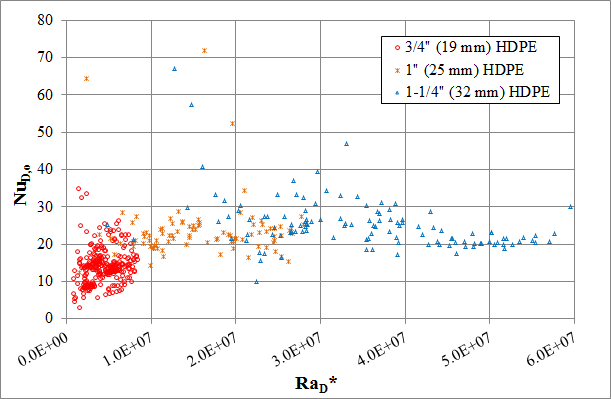
\includegraphics[width=0.8\textwidth]{GarrettsData.png}
		\caption[Heat rejection data collected by \cite{Hansen2011}]{Nusselt vs.\ modified Rayleigh number plot of heat rejection data collected by \cite{Hansen2011}}
		\label{fig:ExpResult:HeatRej:HansenData:NuVsRaGarrettData}
	\end{figure}

In total, 528 data points were collected on 19 spiral-helical SWHE coil configurations by \cite{Hansen2011}. Data collection began on March 2, 2011 and continued through September 2011.

	\subsection{Updated Pond Data Set}
	\label{subsec:ExpResult:HeatRej:UpdatedData}

After the completion of the work performed by \cite{Hansen2011}, an additional 191 data points were collected on eight additional spiral-helical SWHE coil configurations. These additional results, along with the results collected by \cite{Hansen2011} can be seen in Figure \ref{fig:ExpResult:HeatRej:HansenData:AllPondHeatRejData}. These additional tests were collected at the test pond from October 6 through December 2, 2011.

	\begin{figure}
		\centering
		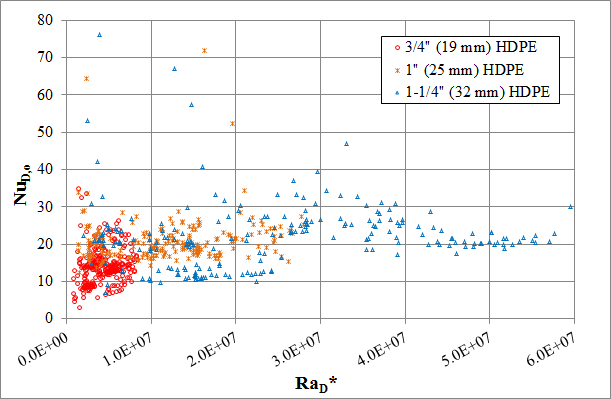
\includegraphics[width=0.8\textwidth]{HeatRejDataBySize.png}
		\caption[Updated pond heat rejection data]{Nusselt vs.\ modified Rayleigh number plot of all heat rejection data collected in the test pond}
		\label{fig:ExpResult:HeatRej:HansenData:AllPondHeatRejData}
	\end{figure}
	
Another summary of the expeimental data can be seen in Table \ref{tab:ExpResult:PondHeatRej:ThermalPercentage} where the average percentage of total thermal resistance for each thermal resistance component is show. Here, we can see that the outside convection resistance makes up on average around 28\% of the total SWHE thermal resistance. The relatively much larger thermal resistance percentage of the SWHE pipe appears to be the area where a small improvement in pipe thermal performance would make the greatest impact.
	
	\begin{table}[h]
		\centering
		\caption[Average thermal resistance percentages for pond heat rejection data]{Average thermal resistance for each thermal resistance component as a percentage of total thermal resistance for pond heat rejection data}
		\label{tab:ExpResult:PondHeatRej:ThermalPercentage}
		\begin{tabular}{p{3cm} c c c c c}
		\hline
		Tube Size & Material & $R_{conv,i}$ & $R_{cond}$ & $R_{conv,o}$ & \# Points\\
		\hline\hline
		3/4 in.\ (19 mm) & PE 3408 & 3.3\% & 63.4\% & 33.3\% & 288\\
		\hline
		1 in.\ (25 mm) & PE 3408 & 2.3\% & 73.3\% & 24.4\% & 199\\
		\hline
		1-1/4 in.\ & \multirow{2}{*}{PE 3408} & \multirow{2}{*}{2.5\%} & \multirow{2}{*}{71.9\%} & \multirow{2}{*}{25.6\%} & \multirow{2}{*}{200} \\
		(32 mm) & & & & \\
		\hline		
		\end{tabular}
	\end{table}

	\subsection{Pool Data}
	\label{subsec:ExpResult:HeatRej:PoolData}

As described in Section \ref{sec:ExpMethod:HeatExtr}, once the weather would not permit heat extraction testing in the test pond, the experiment was moved indoors to the laboratory facility. While there, some additional tests under heat rejection conditions were also performed.

Tests under heat rejection conditions were performed on 3/4 in.\ (19 mm) dia.\ thermally enhanced HDPE with two separate tube-tube spacings. The first was the 2.625 in.\ H x 2.625 in.\ V (67 mm x 67 mm) configuration, and the second was the 2.625 in.\ H x 1.3 in.\ V (67 mm x 33 mm) configuration. 1-1/4 in.\ (32 mm) dia.\ thermally enhanced HDPE was also tested with 4.125 in.\ H x 2.625 in.\ V (105 mm x 67 mm) tube-tube spacings. Nusselt vs.\ modified Rayleigh number plots for these three tests can be seen in Figures \ref{fig:ExpResult:HeatRej:PoolData:Pool_075D_2625H_15V_HeatRej}, \ref{fig:ExpResult:HeatRej:PoolData:Pool_075D_2625H_2626V_HeatRej}, and \ref{fig:ExpResult:HeatRej:PoolData:Pool_125D_4125H_2626V_HeatRej}.

	\begin{figure}
		\centering
		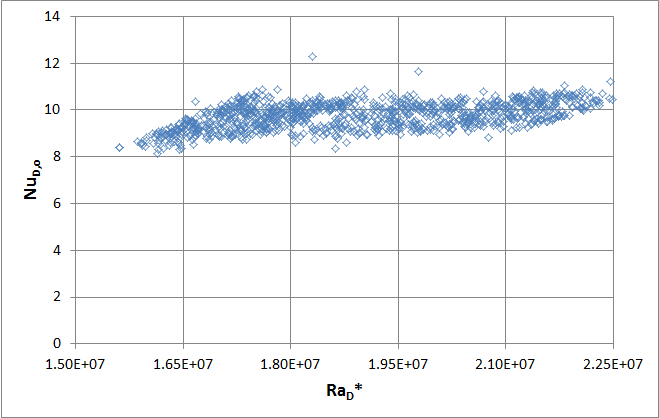
\includegraphics[width=0.8\textwidth]{Pool_075D_2625H_15V_HeatRej.png}
		\caption[Heat rejection data taken in pool on June 30, 2012]{Heat rejection data taken in pool for 3/4 in.\ (19 mm) dia.\ thermally enhanced HDPE for 2.625 in.\ H x 1.3 in.\ V (67 mm x 33 mm) tube-tube spacing}
		\label{fig:ExpResult:HeatRej:PoolData:Pool_075D_2625H_15V_HeatRej}
	\end{figure}	
	
		\begin{figure}
		\centering
		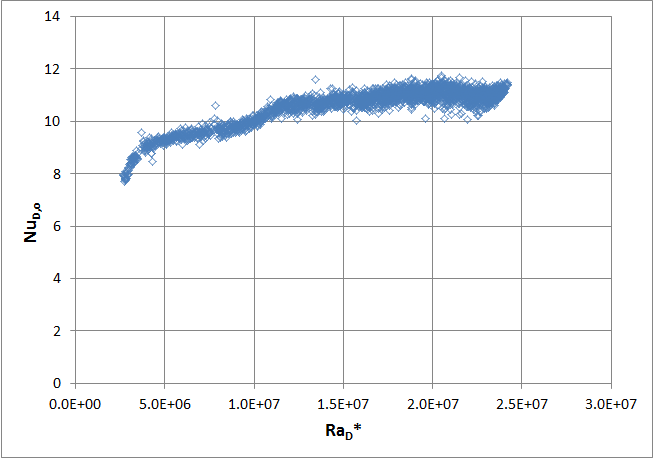
\includegraphics[width=0.8\textwidth]{Pool_075D_2625H_2626V_HeatRej.png}
		\caption[Heat rejection data taken in pool on July 7, 2012]{Heat rejection data taken in pool for 3/4 in.\ (19 mm) dia.\ thermally enhanced HDPE for 2.625 in.\ H x 2.625 in.\ V (67 mm x 67 mm) tube-tube spacing}
		\label{fig:ExpResult:HeatRej:PoolData:Pool_075D_2625H_2626V_HeatRej}
	\end{figure}	
	
		\begin{figure}
		\centering
		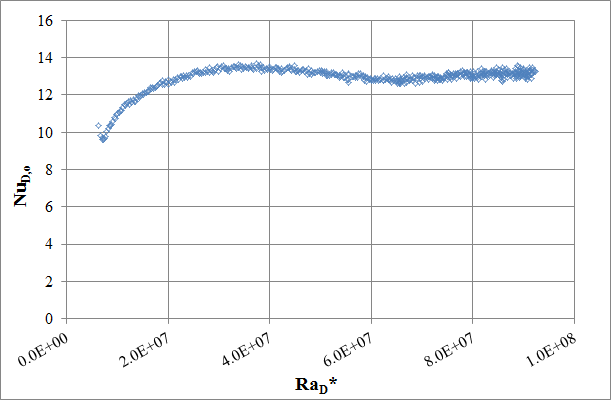
\includegraphics[width=0.8\textwidth]{Pool_125D_4125H_2626V_HeatRej.png}
		\caption[Heat rejection data taken in pool on Oct 24, 2012]{Heat rejection data taken in pool for 1-1/4 in.\ (32 mm) dia.\ thermally enhanced HDPE for 4.125 in.\ H x 2.625 in.\ V (105 mm x 67 mm) tube-tube spacing}
		\label{fig:ExpResult:HeatRej:PoolData:Pool_125D_4125H_2626V_HeatRej}
	\end{figure}
	
Figure \ref{fig:ExpResult:HeatRej:PoolData:Pool_125D_4125H_2626V_HeatRej} shows the Nusselt number begin dropping after about $Ra_D^*=3.5\cdot10^7$. At about $Ra_D^*=6.0\cdot10^7$ we can see separation in the Nusselt numbers. The reason for this dip is not fully understood.

Table \ref{tab:ExpResult:PoolHeatRej:ThermalPercentage} shows the thermal resistance components for each SWHE tube size as a percentage of total thermal resistance. Here, we see that the pipe conduction resistance tends to make up nearly half of the total thermal resistance with the outside convective resistance making up nearly the other half. This shift when compared to the data in Table \ref{tab:ExpResult:PondHeatRej:ThermalPercentage} is theorized to be due to the constrained nature of the pool combined with the fact that the data was taken on thermally enhanced HDPE.

	\begin{table}[h]
		\centering
		\caption[Average thermal resistance percentages for pool heat rejection data]{Average thermal resistance for each thermal resistance component as a percentage of total thermal resistance for pool heat rejection data}
		\label{tab:ExpResult:PoolHeatRej:ThermalPercentage}
		\begin{tabular}{p{3cm} c c c c c}
		\hline
		Tube Size & Material & $R_{conv,i}$ & $R_{cond}$ & $R_{conv,o}$ & \# Points\\
		\hline\hline
		3/4 in.\ (19 mm) & TEHDPE & 4.1\% & 48.1\% & 47.8\% & 3562 \\
		\hline
		1-1/4 in.\ & \multirow{2}{*}{TEHDPE} & \multirow{2}{*}{5.4\%} & \multirow{2}{*}{50.5\%} & \multirow{2}{*}{44.1\%} & \multirow{2}{*}{1420} \\
		(32 mm) & & & & \\
		\hline	
		\end{tabular}
	\end{table}	

\section{Heat Extraction Results}
\label{sec:ExpResult:HeatExtr}
	
	
	\subsection{Pond Data}
	\label{subsec:ExpResult:HeatExtr:PondData}
	
Due to the nature of the testing apparatus, it was not possible to directly vary heat extraction rate. A series of tests were run at steady state conditions for six hours up to two days at a time. Data were collected at varying intervals of one minute up to five minutes. This can be seen below in Figure \ref{fig:ExpResult:HeatExtr:PondData:PlotFeb13} where 24 hours of experimental run time is shown. 

	\begin{figure}
		\centering
		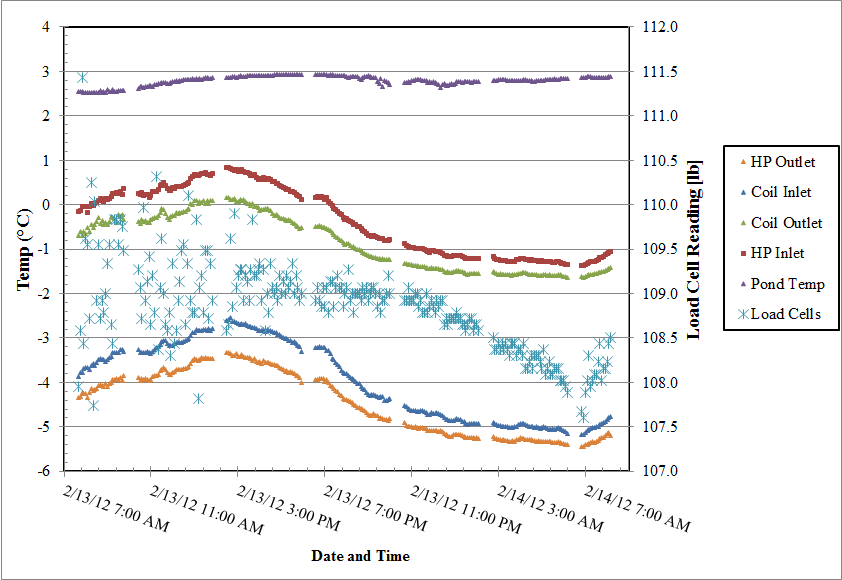
\includegraphics[width=0.8\textwidth]{PlotFeb13.png}
		\caption[Data from heat extraction experiment in test pond]{Data from heat extraction experiment during test in the test pond on February 13, 2012}
		\label{fig:ExpResult:HeatExtr:PondData:PlotFeb13}
	\end{figure}	
	
Also visible in Figure  \ref{fig:ExpResult:HeatExtr:PondData:PlotFeb13} are breaks in the data where gaps can be seen. The water-water heat pump used for the heat extraction tests had a safety feature built in which caused the heat pump to shutdown after four hours of continuous run time. During this time, the heat pump performed diagnostics on itself to verify all safety switches were functioning properly. After a five minute diagnostic period, the heat pump would begin operation again. Due to the disruptions in the run time, the data for up to 40 minute after the beginning of the shut down were cut from the data set. This was done to eliminate the transient affects that were introduced into the system because of the heat pump shutdown. New microchips that control the heat pump run time were ordered, but not installed until the experiment had been moved to the indoor test facility.


The signal output directly from the load cells can also be seen in Figure \ref{fig:ExpResult:HeatExtr:PondData:PlotFeb13}. A decrease in load cell output indicates an increase in buoyancy force, potentially signifying ice formation. On this occasion, the load cells recorded approximately 1.5 lb.\ (6.7 N) decrease in load cell reading which may be attributed to ice formation on the coil. Consequently, this was the only recorded potential ice formation that occurred while running experiments in the pond. The summer and winter of 2011-2012 were among the warmest on record. Due to that, it is uncertain if any ice was formed on the coil while running experiments in the pond. Photos of the test data corresponding to Figure \ref{fig:ExpResult:HeatExtr:PondData:PlotFeb13} can be seen in Figures \ref{fig:ExpResult:HeatExtr:PondData:Photo1Feb13} and \ref{fig:ExpResult:HeatExtr:PondData:Photo2Feb13}.
	
	\begin{figure}
		\centering
		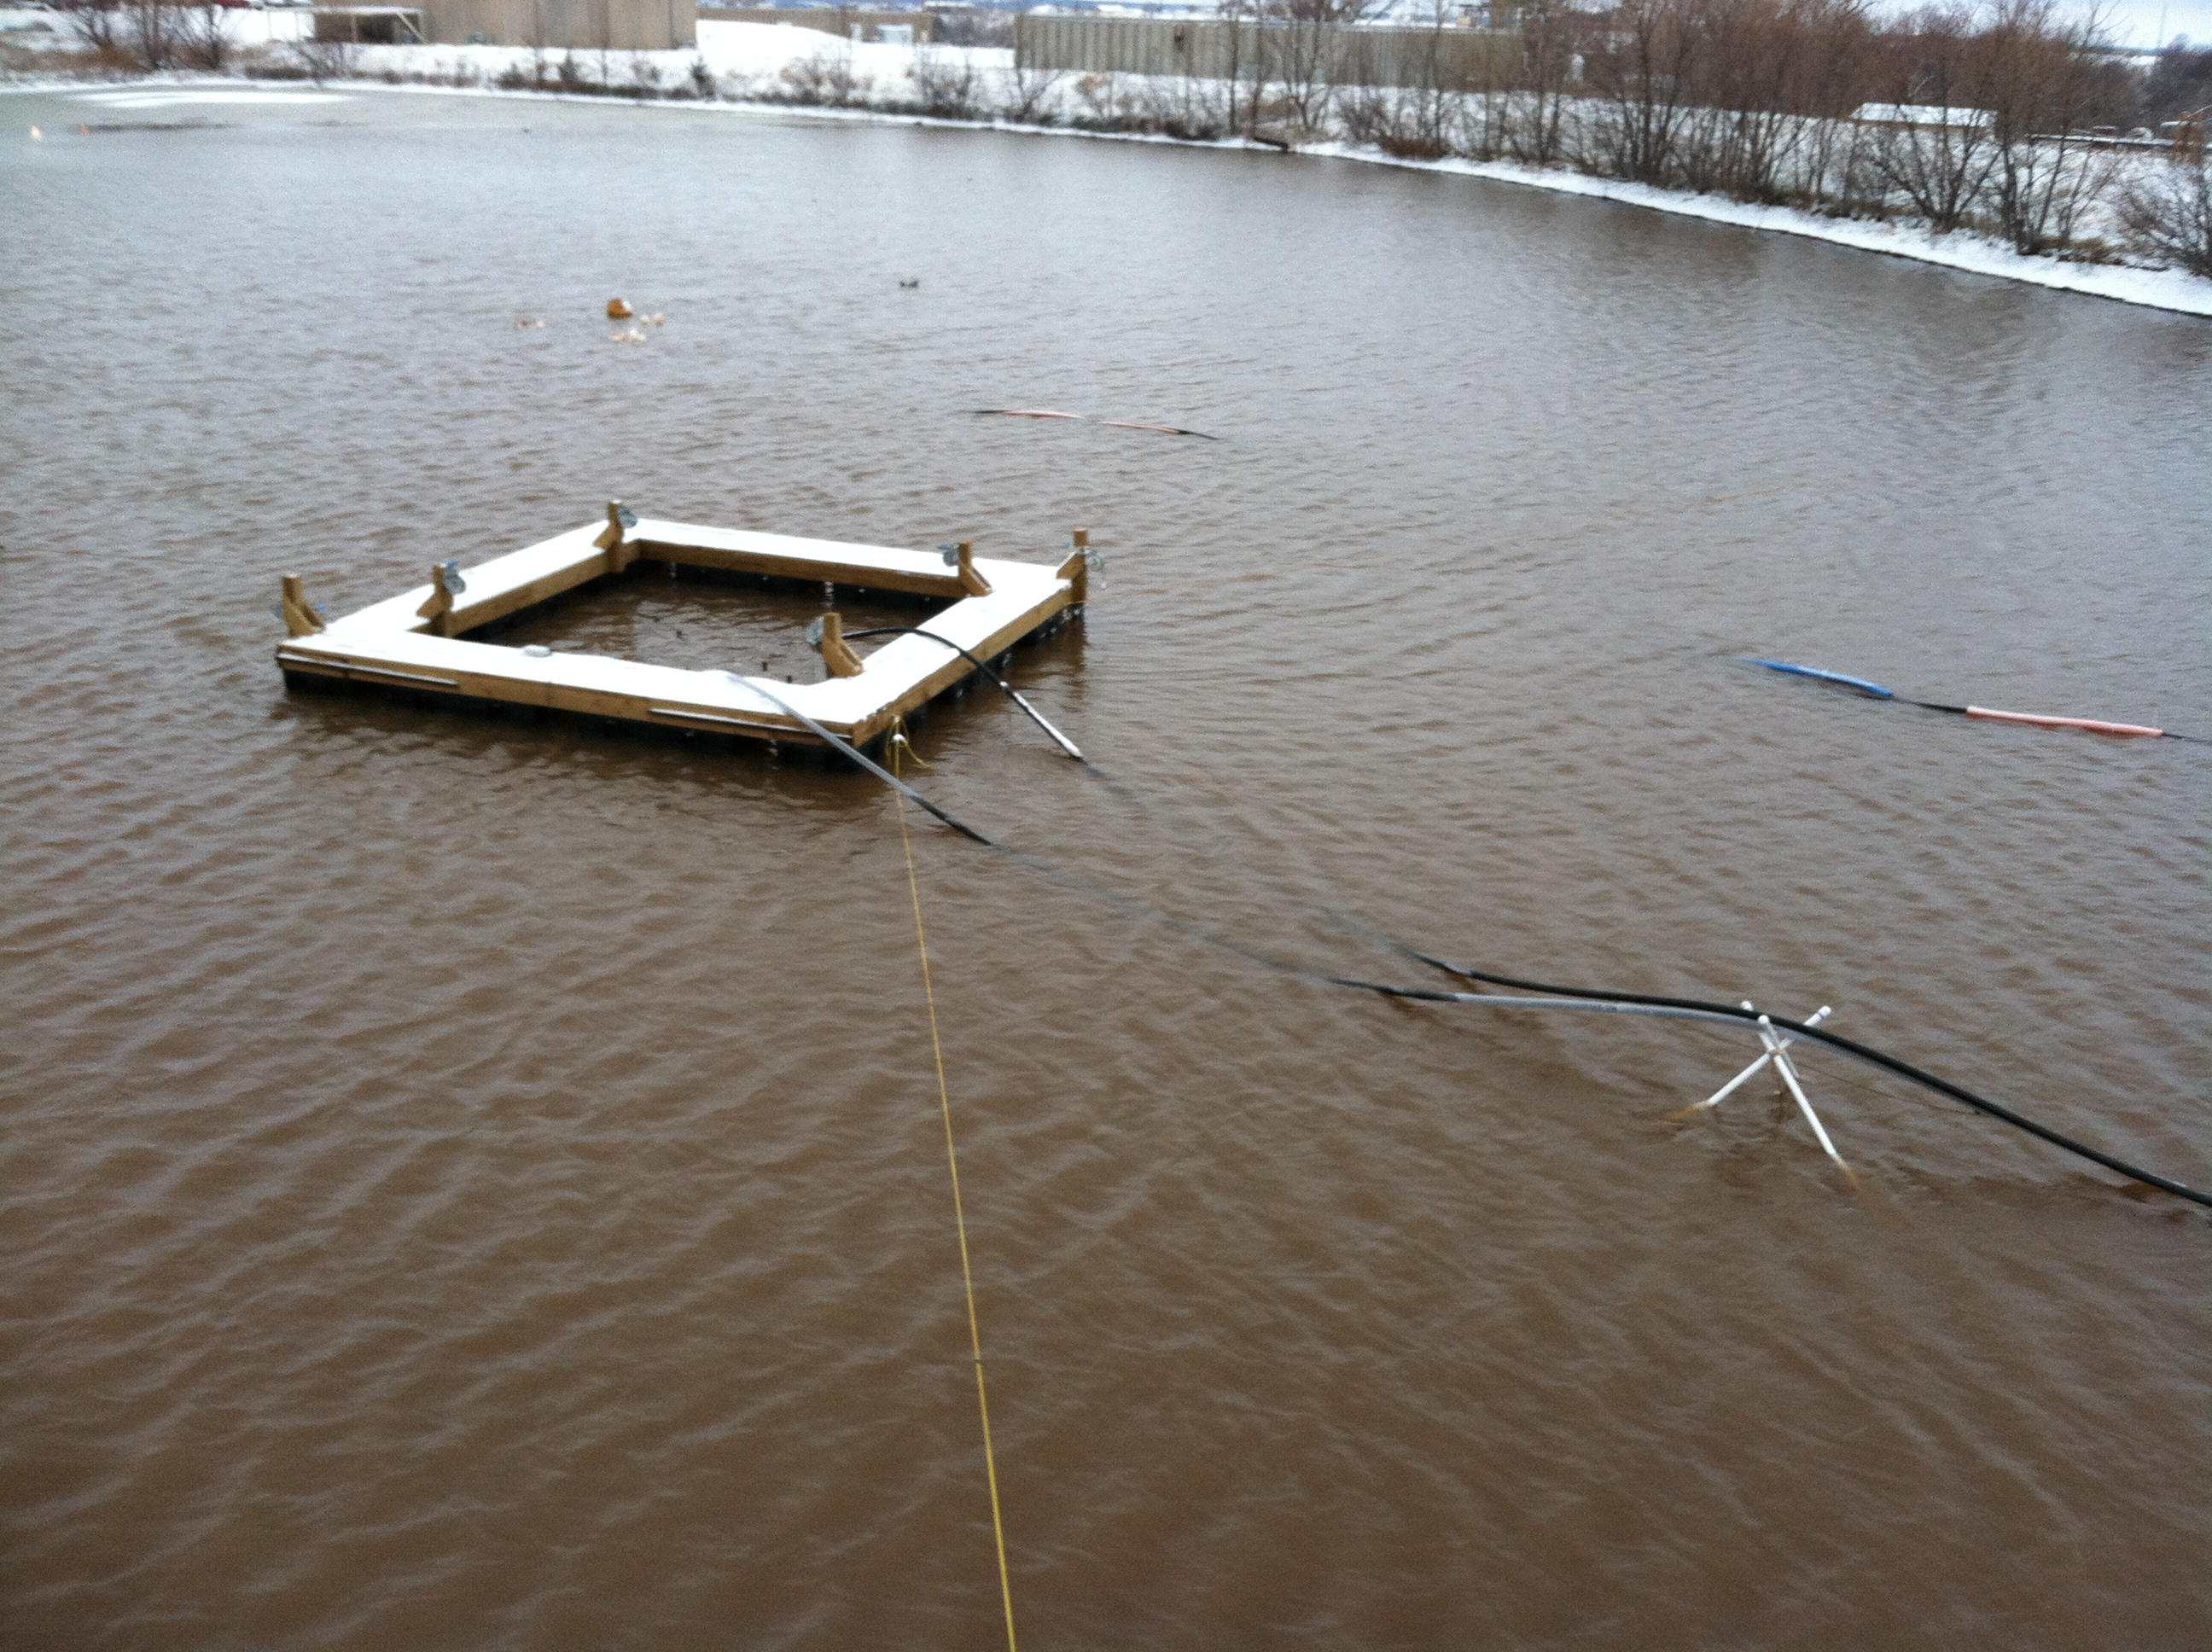
\includegraphics[width=0.8\textwidth]{Photo1Feb13.jpg}
		\caption[Heat extraction platform in pond during test]{Heat extraction platform during heat extraction test in the test pond on February 13, 2012}
		\label{fig:ExpResult:HeatExtr:PondData:Photo1Feb13}
	\end{figure}	
	
	\begin{figure}
		\centering
		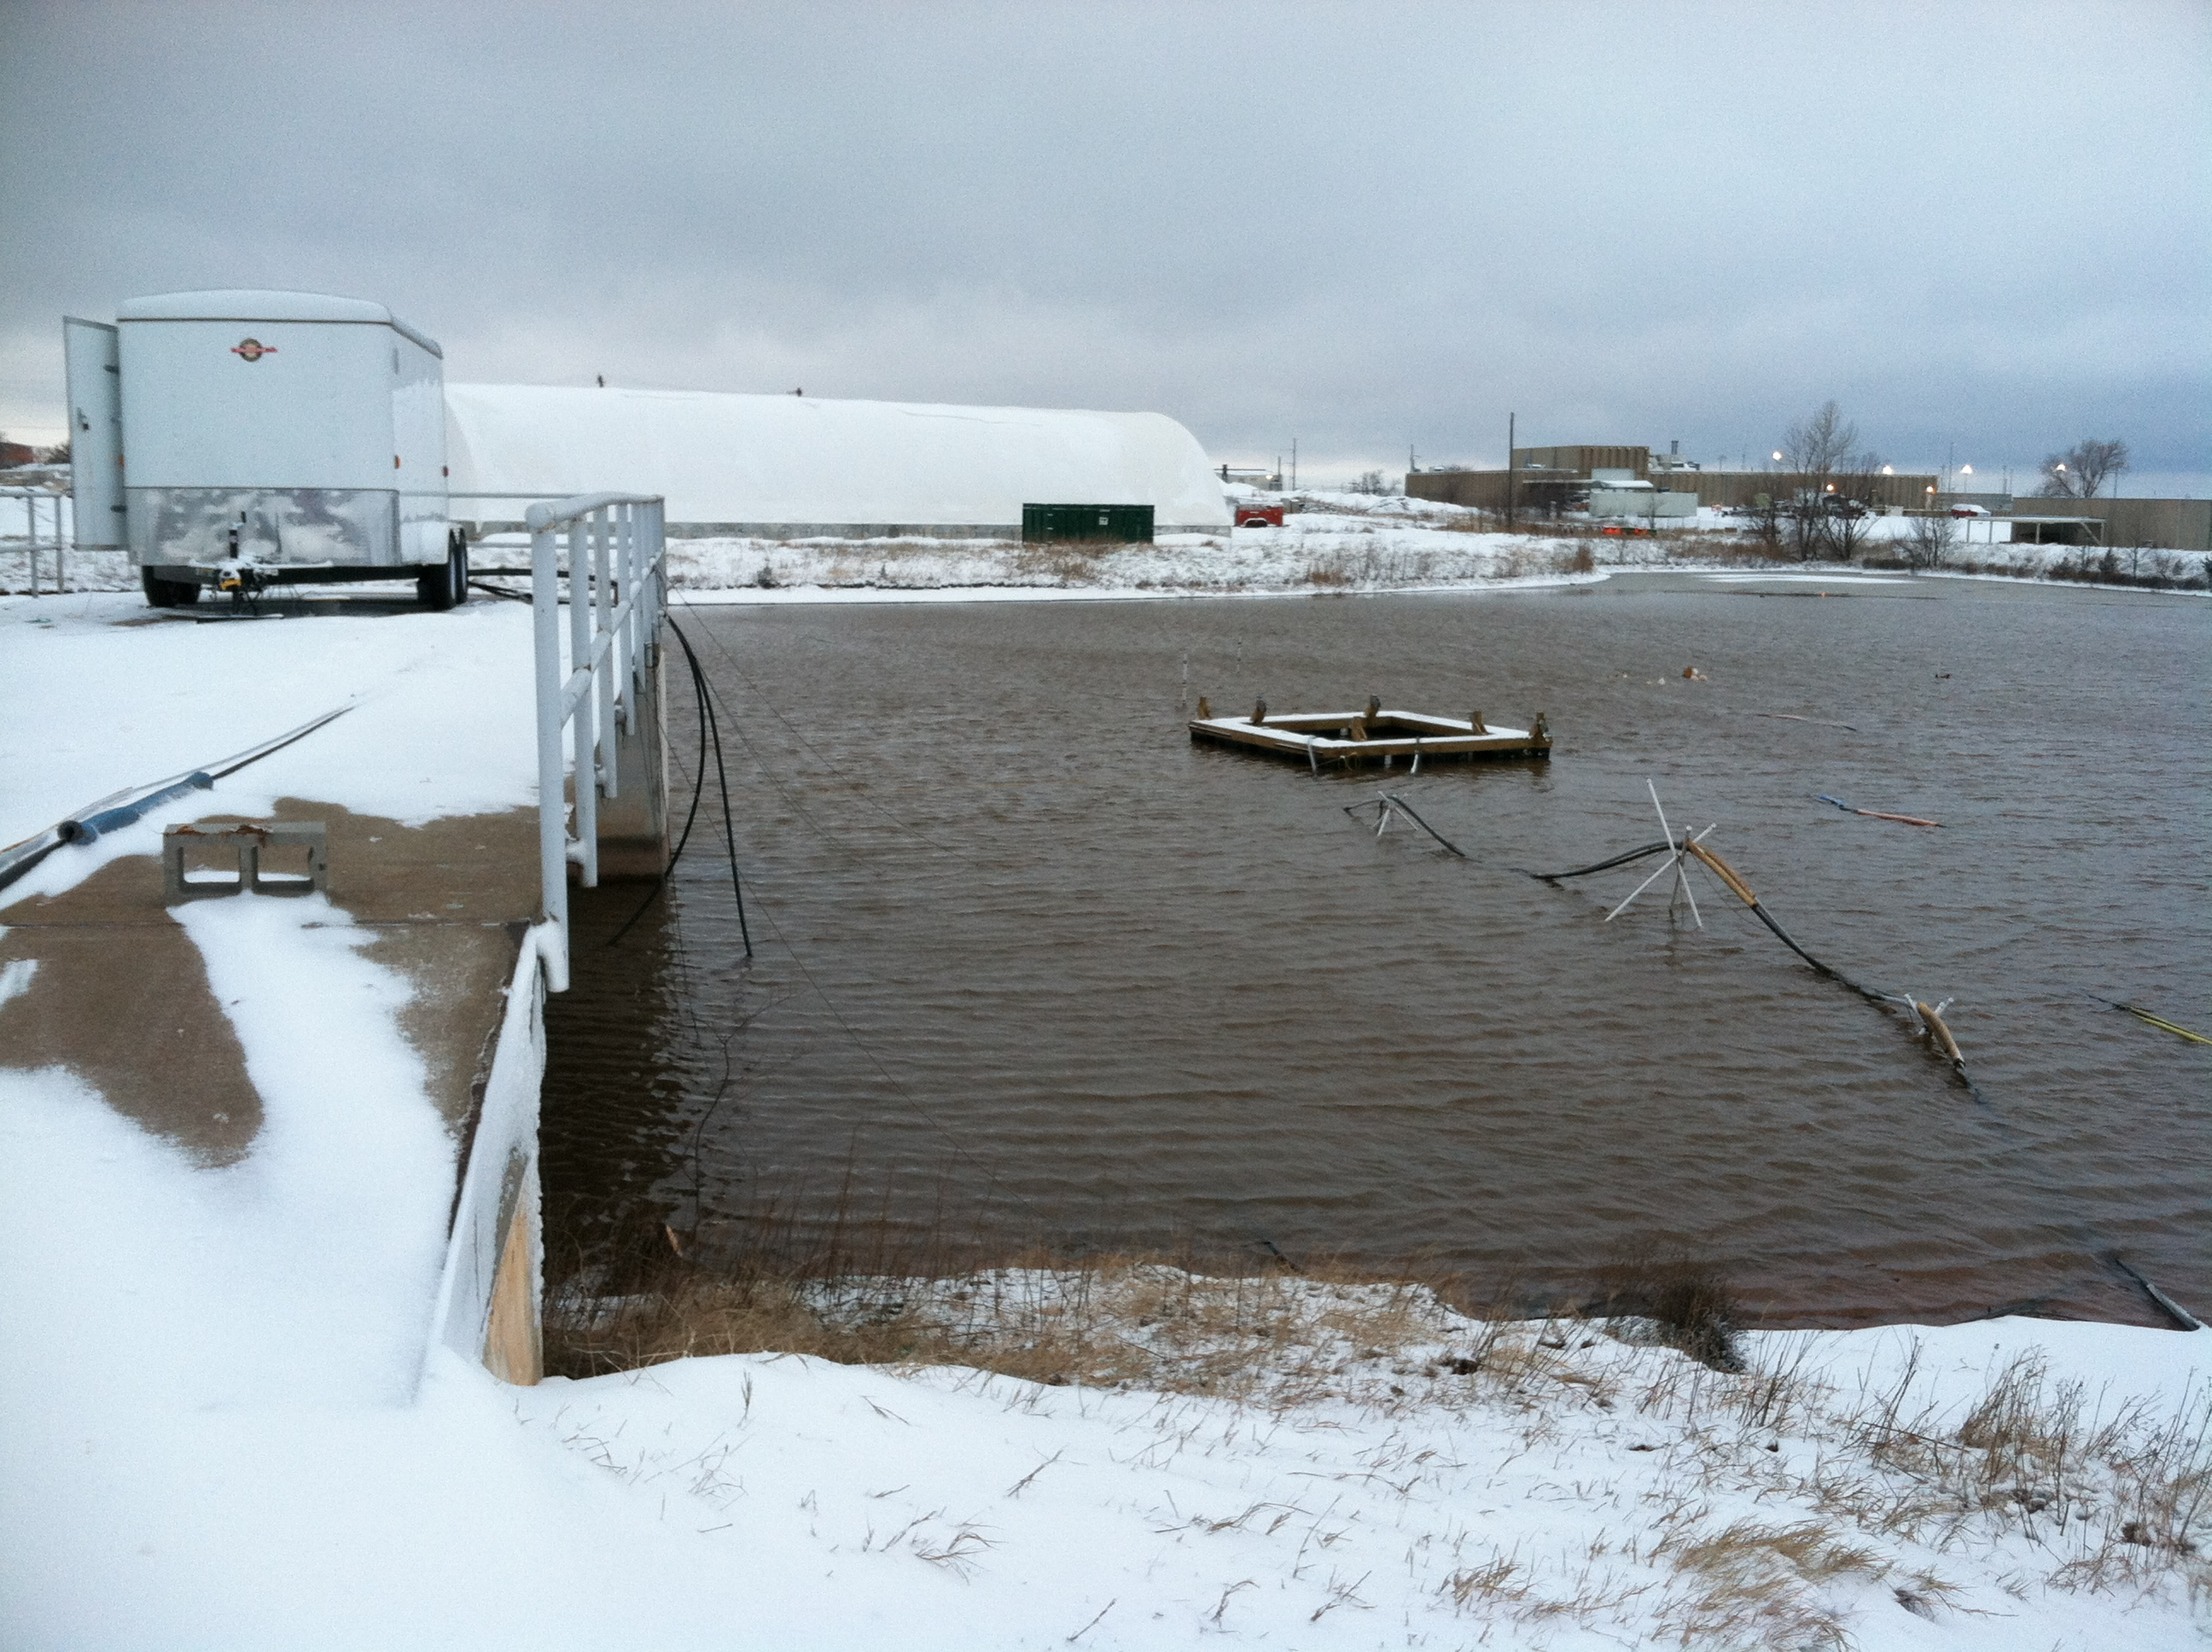
\includegraphics[width=0.8\textwidth]{Photo2Feb13.jpg}
		\caption[Heat extraction experiment in pond during test]{Heat extraction experiment during test in the test pond on February 13, 2012}
		\label{fig:ExpResult:HeatExtr:PondData:Photo2Feb13}
	\end{figure}	

All heat extraction data collected in the test pond can be seen in Figure \ref{fig:ExpResult:HeatExtr:PondData:PondHeatExtractionData}. In order to collect the pond data, a series of tests were performed from January 19, 2012 to March 9, 2012. All data collected in the pond under heat extraction conditions was taken on  thermally enhanced 3/4 in.\ (19 mm) dia.\ SDR-11 HDPE pipe. The coil length was 500 ft (152.4 m) and the tubes were arranged on horizontal and vertical tube-tube spacing of 2.625 in.\ H x 2.625 in.\ V (67 mm x 67 mm). 
	
	\begin{figure}
		\centering
		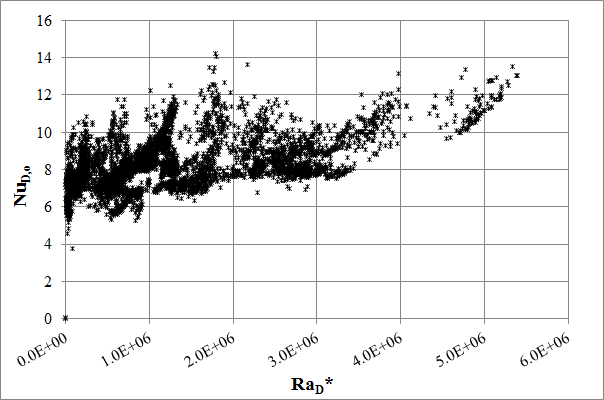
\includegraphics[width=0.8\textwidth]{PondHeatExtractionData.png}
		\caption[Pond heat extraction data taken on February 13, 2011]{Nusselt vs.\ modified Rayleigh number plot of heat extraction data collected in the test pond}
		\label{fig:ExpResult:HeatExtr:PondData:PondHeatExtractionData}
	\end{figure}
	
Table \ref{tab:ExpResult:PondHeatExtr:ThermalPercentage} shows the thermal resistance of each resistance component as a percentage of the total thermal resistance. Because the pond heat extraction data was taken on thermally enhanced pipe, the pipe conduction resistance represents a smaller portion of the total thermal resistance. When comparing with the same data for the 3/4 in.\ (19 mm) pipe in Table \ref{tab:ExpResult:PondHeatRej:ThermalPercentage}, the more conductive pipe causes the outside convective resistance to go from 33\% up to 54\%.

	\begin{table}[h]
		\centering
		\caption[Average thermal resistance percentages for pond heat extraction data]{Average thermal resistance for each thermal resistance component as a percentage of total thermal resistance for pond heat extraction data}
		\label{tab:ExpResult:PondHeatExtr:ThermalPercentage}
		\begin{tabular}{p{3cm} c c c c c}
		\hline
		Tube Size & Material & $R_{conv,i}$ & $R_{cond}$ & $R_{conv,o}$ & \# Points\\
		\hline\hline
		3/4 in.\ (19 mm) & TEHDPE & 6.1\% & 39.5\% & 54.4\% & 5350\\
		\hline	
		\end{tabular}
	\end{table}
 
	\subsection{Pool Data}
	\label{subsec:ExpResult:HeatExtr:PoolData}
	
Once the experiment was moved indoors, heat extraction data was collected in the pool. Figures \ref{fig:ExpResult:HeatExtr:PoolData:Pool_075D_2625H_15V_HeatExtr}, \ref{fig:ExpResult:HeatExtr:PoolData:Pool_075D_2625H_2626V_HeatExtr}, and \ref{fig:ExpResult:HeatExtr:PoolData:Pool_125D_4125H_2626V_HeatExtr} show the heat extraction test data for three different coil configurations. All tests were run on thermally enhanced HDPE pipe with a coil length of 500 ft (152.4 m). Periods where coil icing occurred were filtered from the data sets for external convection calculation purposes. Points labeled a), b), c) and d) in Figure \ref{fig:ExpResult:HeatExtr:PoolData:Pool_075D_2625H_15V_HeatExtr} will be described in the subsequent paragraphs and illustrated with Figure \ref{fig:ExpResult:HeatExtr:PoolData:DensityPoints}.

	\begin{figure}
		\centering
		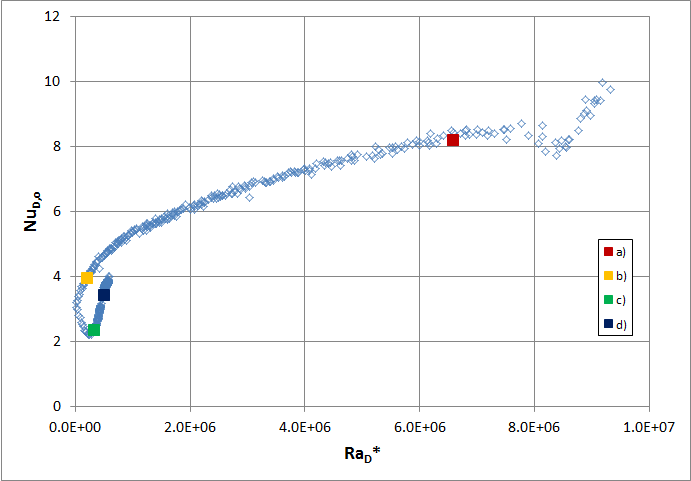
\includegraphics[width=0.8\textwidth]{Pool_075D_2625H_15V_HeatExtr.png}
		\caption[Heat extraction data taken in pool on June 21, 2012.]{Heat extraction data taken in pool for 3/4 in.\ (19 mm) dia.\ thermally enhanced HDPE for 2.625 in.\ H x 1.3 in.\ V (67 mm x 33 mm) tube-tube spacing}
		\label{fig:ExpResult:HeatExtr:PoolData:Pool_075D_2625H_15V_HeatExtr}
	\end{figure}	
	
		\begin{figure}
		\centering
		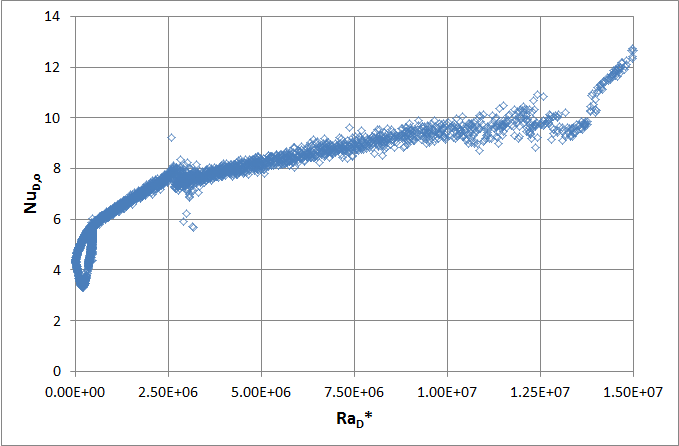
\includegraphics[width=0.8\textwidth]{Pool_075D_2625H_2626V_HeatExtr.png}
		\caption[Heat extraction data taken in pool on August 6, 2012.]{Heat extraction data taken in pool for 3/4 in.\ (19 mm) dia.\ thermally enhanced HDPE for 2.625 in.\ H x 2.625 in.\ V (67 mm x 67 mm) tube-tube spacing}
		\label{fig:ExpResult:HeatExtr:PoolData:Pool_075D_2625H_2626V_HeatExtr}
	\end{figure}	
	
		\begin{figure}
		\centering
		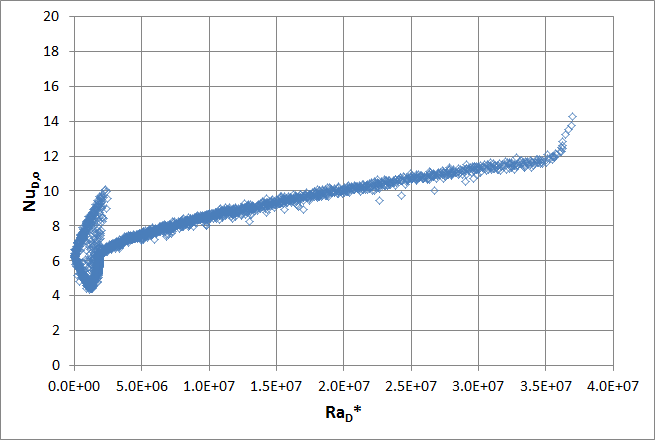
\includegraphics[width=0.8\textwidth]{Pool_125D_4125H_2626V_HeatExtr.png}
		\caption[Heat extraction data taken in pool on Oct 22, 2012.]{Heat extraction data taken in pool for 1-1/4 in.\ (32 mm) dia.\ thermally enhanced HDPE for 4.125 in.\ H x 2.625 in.\ V (105 mm x 67 mm) tube-tube spacing}
		\label{fig:ExpResult:HeatExtr:PoolData:Pool_125D_4125H_2626V_HeatExtr}
	\end{figure}	
	
From Figures \ref{fig:ExpResult:HeatExtr:PoolData:Pool_075D_2625H_15V_HeatExtr}, \ref{fig:ExpResult:HeatExtr:PoolData:Pool_075D_2625H_2626V_HeatExtr},
and \ref{fig:ExpResult:HeatExtr:PoolData:Pool_125D_4125H_2626V_HeatExtr}, we see several trends in the data that are worth noting: 

The first is the trend shown near the right side of each plot where the slope of the data is much steeper than the majority of the data. This region represents the data taken during the initial startup period of the test. As the tests began, we can follow the data generated by following from the right side of each chart towards the lower left corner of each chart. This irregular data indicated at the right of each chart shows the initial period where the system is starting up and initial system transients are settling. 

The second trend that should be highlighted is the irregular data shown near the left side of the charts. The reason for this is identified as the region where the density difference between the SWHE cold water plume and the surface water reverses. This occurs due to the maximum density of water which occurs at a temperature of 39.2$^\circ$F (4$^\circ$C) for pure water. In this region, the cold water plume that would be falling from the coil, changes direction and begins flowing upward. To illustrate this, if the SWHE cold water plume had a temperature of 40$^\circ$F (4.4$^\circ$C) and the surface water had a temperature of 45$^\circ$F (7.2$^\circ$C), the cold water plume would be more dense than the surface water and would naturally fall downward. The same could be said if the SWHE cold water plume were 38$^\circ$F (3.3$^\circ$C) with a 45$^\circ$F (7.2$^\circ$C) surface water temperature. However, if the SWHE plume were at a temperature of 33$^\circ$F (0.6$^\circ$C) and the surface water temperature were at 39$^\circ$F (3.9$^\circ$C), the SWHE cold water plume would flow upward. 
	
This is illustrated in Figure \ref{fig:ExpResult:HeatExtr:PoolData:DensityPoints} where the water density in $kg/m^3$ is plotted as a function of temperature in $^\circ$C. Here, the previous point is illustrated to show the change in direction of the SWHE buoyancy plume. At point a) in Figures \ref{fig:ExpResult:HeatExtr:PoolData:Pool_075D_2625H_15V_HeatExtr} and \ref{fig:ExpResult:HeatExtr:PoolData:DensityPoints}, the SWHE plume density taken at the outside film temperature (Equation \ref{eq:ExpResult:HeatRej:DataAnalysis:Tfilmo}) is greater than the pool water density taken at the pool temperature. This density imbalance is the driving force for natural convection. At point a) we can see that the density difference between plume and pool is significant, which corresponds to a higher Nusselt number in Figure \ref{fig:ExpResult:HeatExtr:PoolData:Pool_075D_2625H_15V_HeatExtr}. 
	
	\begin{figure}
		\centering
		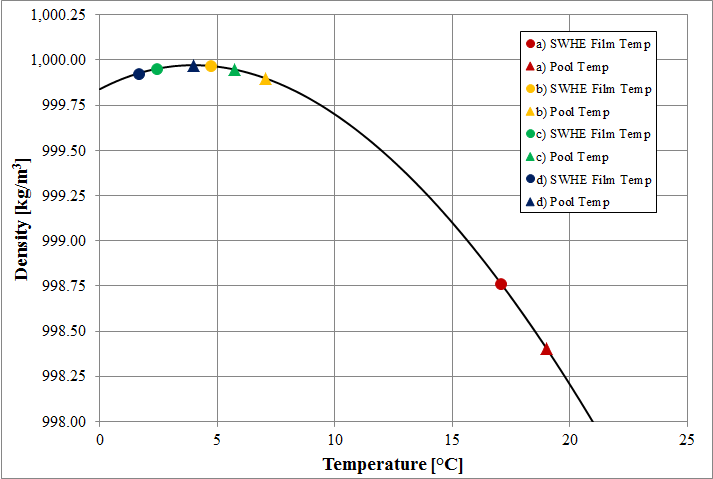
\includegraphics[width=0.8\textwidth]{DensityPoints.png}
		\caption{Points illustrating the buoyancy plume direction change in Figure \ref{fig:ExpResult:HeatExtr:PoolData:Pool_075D_2625H_15V_HeatExtr}}
		\label{fig:ExpResult:HeatExtr:PoolData:DensityPoints}
	\end{figure}
	
As we move from point a) to b), the density difference between the two points is quite small, resulting in smaller Nusselt numbers in Figure \ref{fig:ExpResult:HeatExtr:PoolData:Pool_075D_2625H_15V_HeatExtr}. Point c) illustrates a balance point where the density of the plume and the pool water are nearly equal, resulting in Nusselt numbers which are at the lowest point in Figure \ref{fig:ExpResult:HeatExtr:PoolData:Pool_075D_2625H_15V_HeatExtr}. This is also the point where the flow direction is changing. Finally, as we move to point d), the plume density is now less than the pool water signifying an upwardly buoyant plume.
	
Due to the fact that the SWHE is quite long (500 ft (152.4 m)), different locations along the tube length are expected to make this flow direction transition at different points in time. Because circulating fluid enters the heat exchanger at the bottom and exits at the top, the plume would transition to upward flow near the bottom of the SWHE before the upper layers would transition to upward flow. Other scenarios are likely as well.

I hypothesize that due to these two competing flow directions associated with different locations along the tube passing through the maximum density point at different times, we see the external convective resistance increases substantially. Once the majority of the SWHE has transitioned to the upward flow regime, the external convective resistance is shown to decrease again. The lowest Nusselt number could be considered a ``balance" point where we have similar magnitudes of upward and downward flow.
	
There is also some apparent hysteresis in the data as it passes through the maximum density point. I hypothesize this is due to the fact that with a downward flow, the coldest water settles at the bottom of the pool with little recirculation occurring. However, for the upward flow regime we will see that the coldest water will rise to the pool surface. As that water warms, it will then settle to the bottom of the pool and a recirculation zone will form. As a result of the physics associated with the various flow patterns, we expect to see hysteresis in the data near the maximum density point.

Table \ref{tab:ExpResult:PoolHeatExtr:ThermalPercentage} shows the percentages of total thermal resistance each thermal resistance component makes up for this particular set of experimental data. The external convective resistance is greater, when compared to the percentages of total thermal resistance components for the pond heat rejection data from Table \ref{tab:ExpResult:PondHeatExtr:ThermalPercentage}. Again, this is theorized to be due to the constrained nature of the pool.

	\begin{table}[h]
		\centering
		\caption[Average thermal resistance percentages for pool heat extraction data]{Average thermal resistance for each thermal resistance component as a percentage of total thermal resistance for pool heat extraction data}
		\label{tab:ExpResult:PoolHeatExtr:ThermalPercentage}
		\begin{tabular}{p{3cm} c c c c c}
		\hline
		Tube Size & Material & $R_{conv,i}$ & $R_{cond}$ & $R_{conv,o}$ & \# Points\\
		\hline\hline
		3/4 in.\ (19 mm) & TEHDPE & 5.8\% & 32.2\% & 62.0\% & 4725 \\
		\hline
		1-1/4 in.\ & \multirow{2}{*}{TEHDPE} & \multirow{2}{*}{6.1\%} & \multirow{2}{*}{35.1\%} & \multirow{2}{*}{58.8\%} & \multirow{2}{*}{3149} \\		
		(32 mm) & & & & & \\
		\hline	
		\end{tabular}
	\end{table}	

 
\subsection{Coil Icing}
\label{subsec:ExpResult:HeatExtr:CoilIcing}

The main purpose of moving the experiment to the indoor facility was to collect information regarding SWHE performance under heat extraction and coil icing conditions. Because there was only one test where ice was potentially formed on the coil while running in the pond, the data considered in this section will be taken from the heat extraction tests in the pool.

Shown in Figure \ref{fig:ExpResult:HeatExtr:CoilIcing:FrozenCoil} is a SWHE during a heat extraction test under fully iced conditions. The SWHE had the 2.625 in.\ H x 1.3 in.\ V (67 mm x 33 mm) tube-tube configurations on 3/4 in.\ (19 mm) SDR-11 thermally enhanced HDPE piping. In this figure, we can see that the lead pipes bringing circulating fluid to/from the SWHE are iced with frost. Looking closely we can see the ice layers that had formed on the SWHE.

	\begin{figure}
		\centering
		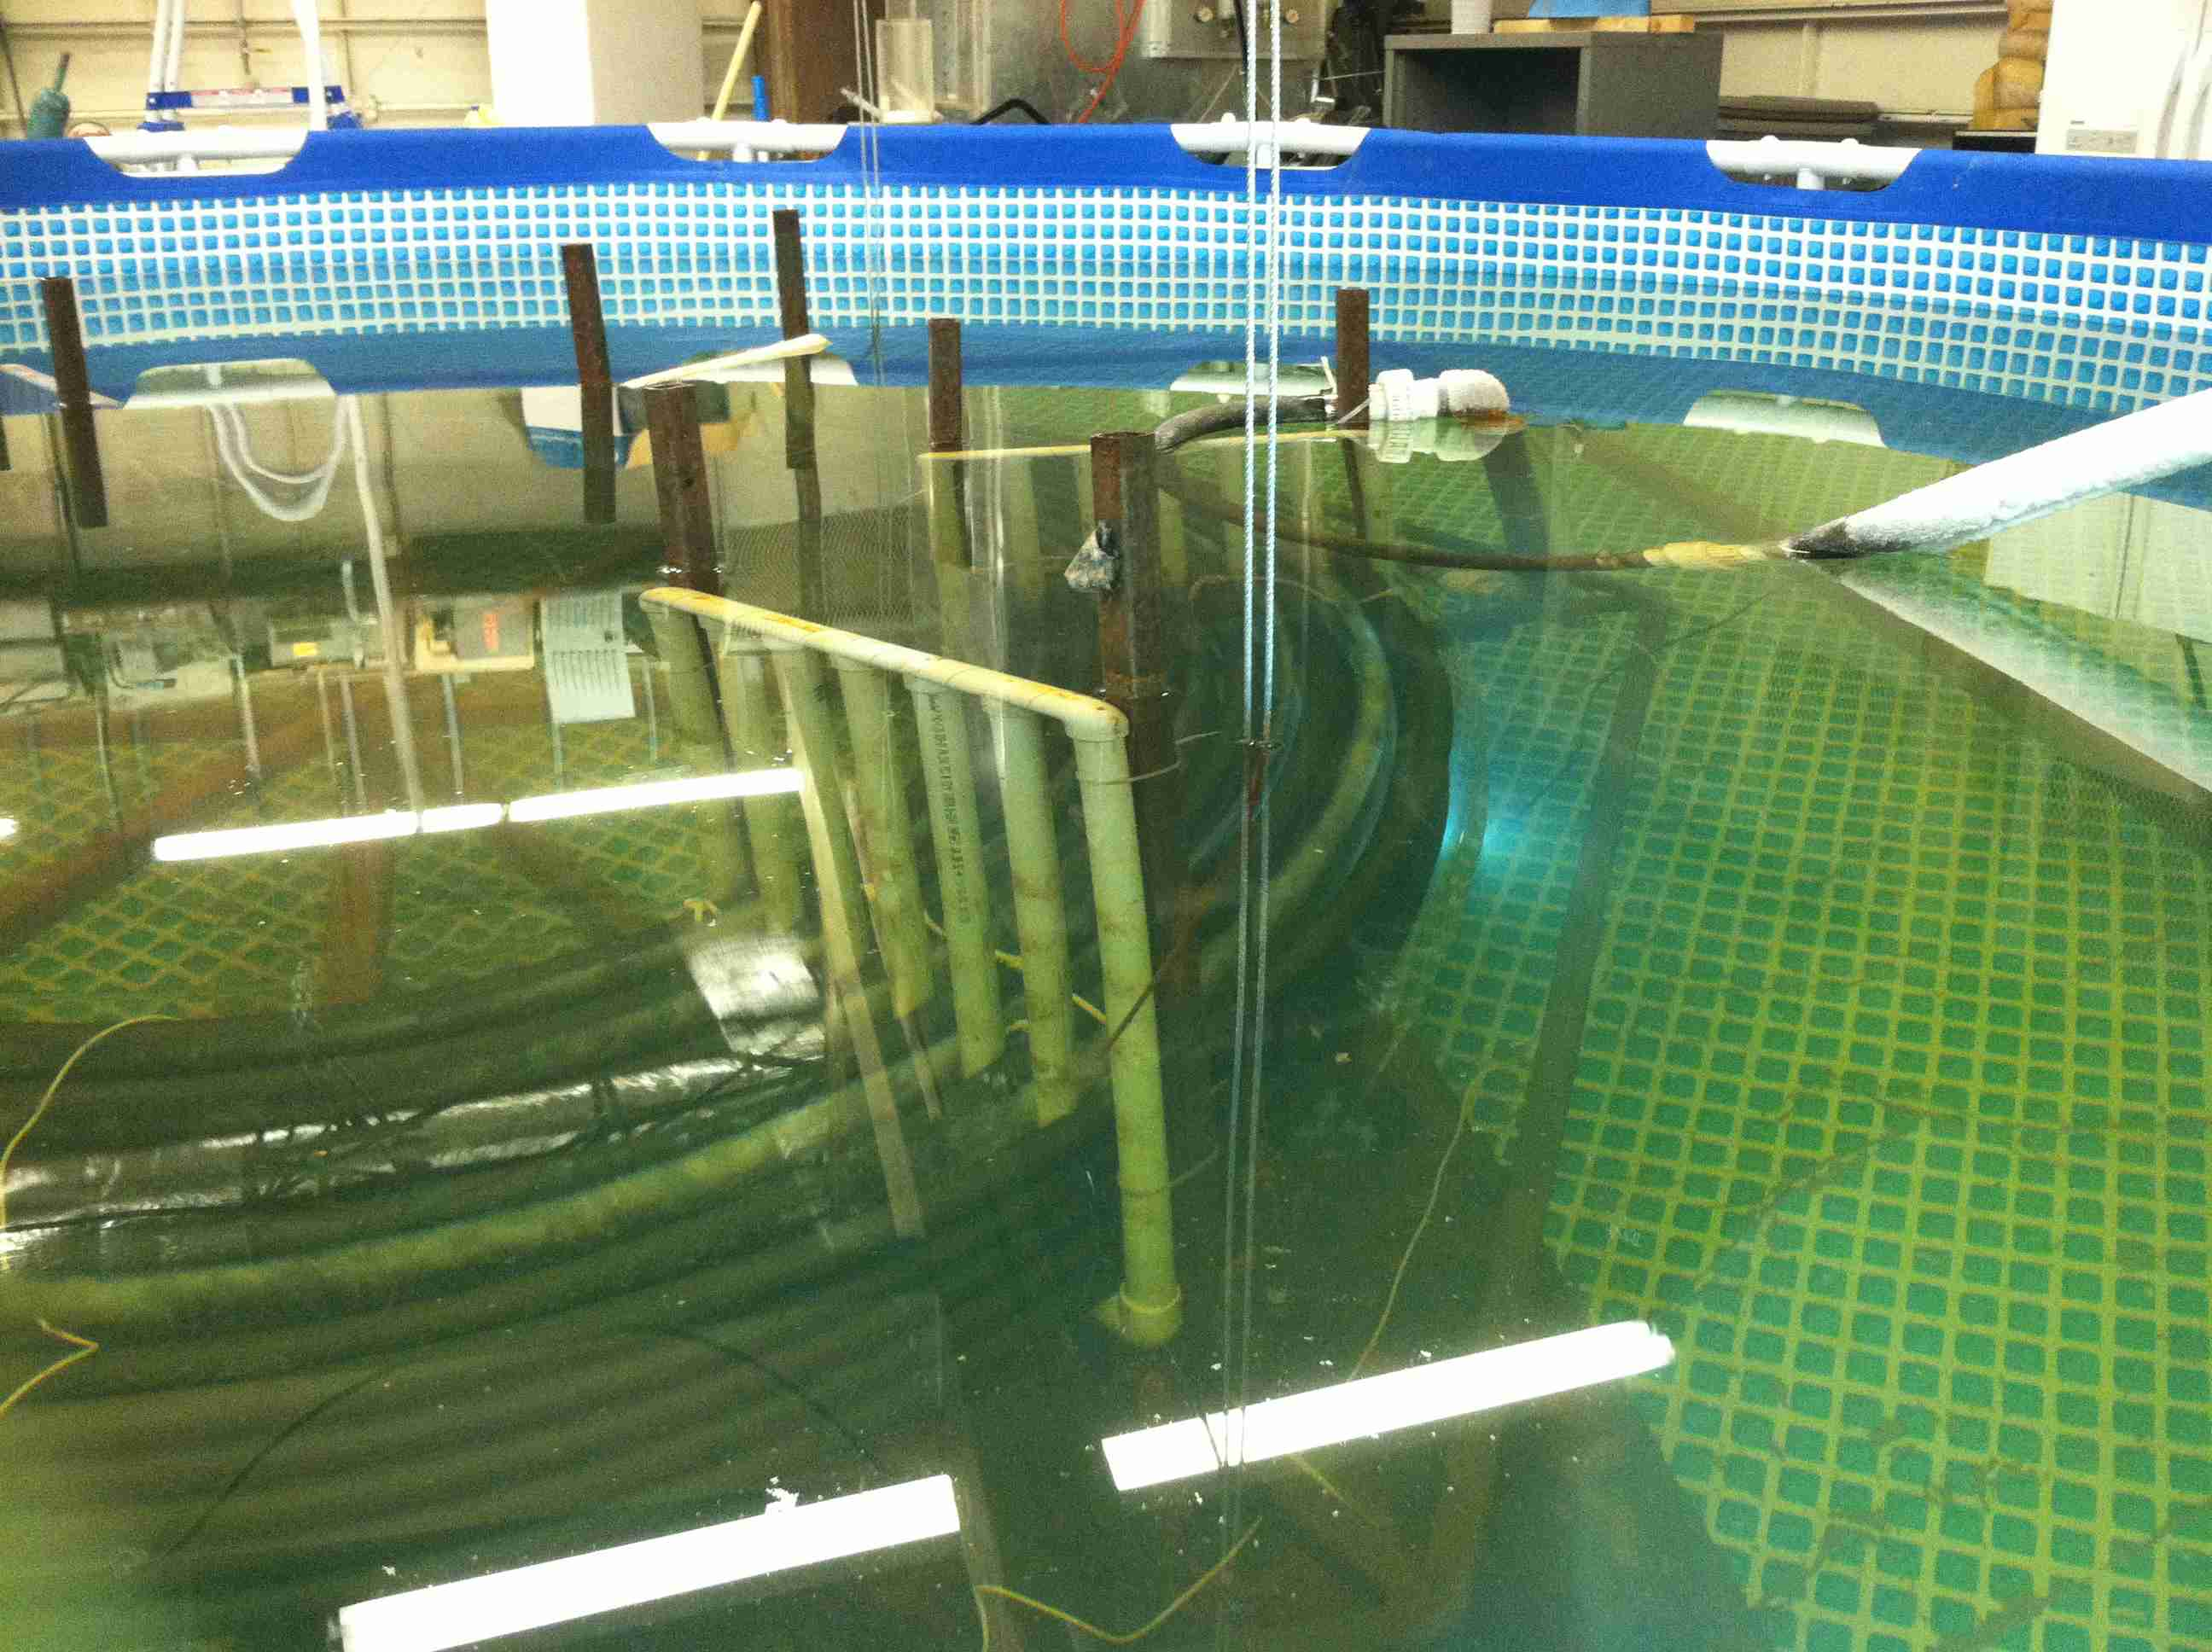
\includegraphics[width=0.8\textwidth]{FrozenCoil.JPG}
		\caption[Fully iced surface water heat exchanger]{3/4 in.\ dia.\ (19 mm) 2.625 in.\ H x 1.3 in.\ V (67 mm x 33 mm) SWHE that is fully iced}
		\label{fig:ExpResult:HeatExtr:CoilIcing:FrozenCoil}
	\end{figure}

Figure \ref{fig:ExpResult:HeatExtr:CoilIcing:PoolIcingPlot1} below shows some of the data collected from the coil shown above in Figure \ref{fig:ExpResult:HeatExtr:CoilIcing:FrozenCoil} during the heat extraction test. Entering and exiting circulating fluid temperatures are shown, as well as the pool water temperature averaged across the depth of the heat exchanger. Also shown is the buoyancy force created from the ice formation on the SWHE. The buoyancy force peaks near 62 lb.\ (276 N). From the plot, we see that the coil temperatures begin to drop sharply as a direct result of the additional thermal resistance due to the ice formation. 

The step in SHWE entering and exiting temperature after the SWHE is fully iced is the point where the large three ton (10.6 kW) heat pump was turned off while leaving the smaller one ton (3.5 kW) heat pump on. At this point, the coil was fully iced and buoyancy force was not increasing. Due to the limitations of the current system, the large heat pump was switched off to allow for coil deicing.

	\begin{figure}
		\centering
		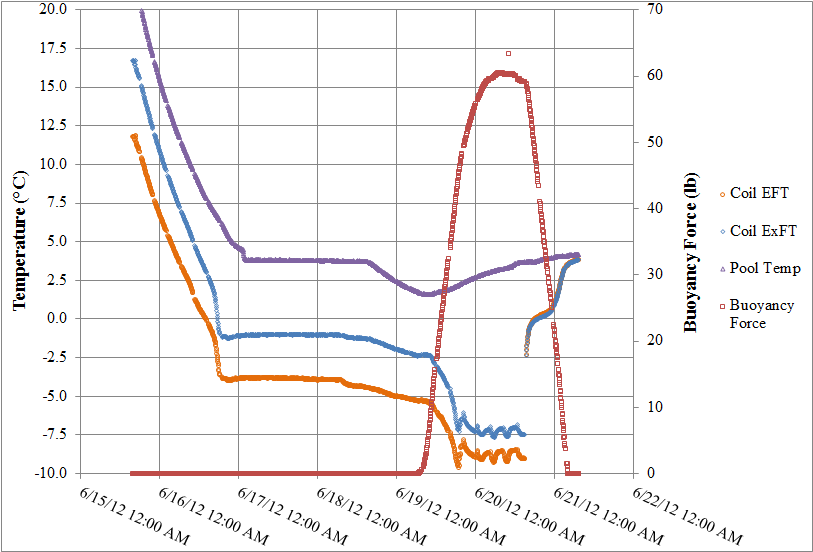
\includegraphics[width=0.8\textwidth]{PoolIcingPlot1.png}
		\caption[Coil temperature and buoyancy force from coil icing test on the 3/4 in.\ dia.\ (19 mm) 2.625 in.\ H x 1.3 in.\ V (67 mm x 33 mm) coil]{Coil temperature and buoyancy force plot from test in pool on 3/4 in.\ dia.\ (19 mm) 2.625 in.\ H x 1.3 in.\ V (67 mm x 33 mm) SDR-11 thermally enhanced HDPE}
		\label{fig:ExpResult:HeatExtr:CoilIcing:PoolIcingPlot1}
	\end{figure}

We can also see the pool temperatures begin to rise at the onset of ice formation. This occurs due to the decreased heat extraction rate which occurs after ice begins forming on the tubes. This increase in pool temperature is the natural result of the decreased heat transfer rate combined with heat gain through the pool boundaries.

In Figure \ref{fig:ExpResult:HeatExtr:CoilIcing:PoolIcingPlot2}, we can see the coil heat transfer rate in conjunction with the buoyancy force. If we examine the graph relatively close, we can see that heat transfer continues at relatively the same level after the onset of ice formation when compared to the period of time immediately previous the onset of ice formation. The slope of the buoyancy force is also relatively constant.

	\begin{figure}
		\centering
		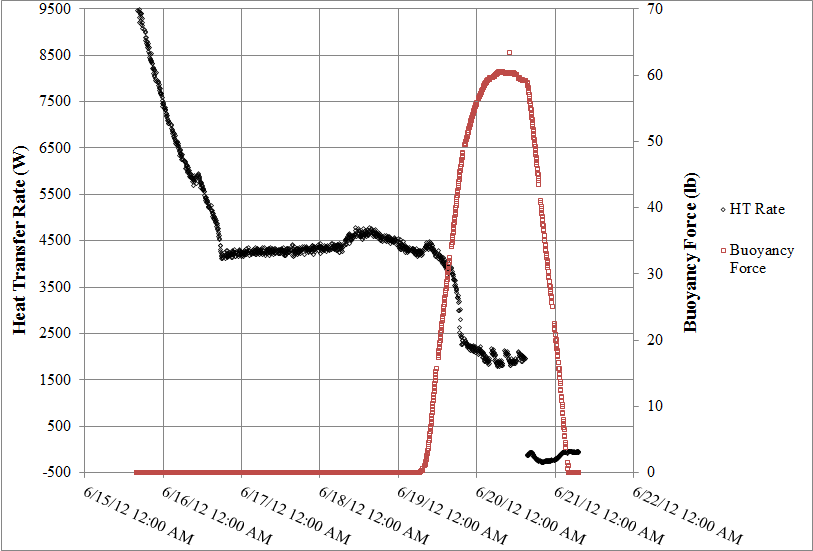
\includegraphics[width=0.8\textwidth]{PoolIcingPlot2.png}
		\caption[Coil heat transfer rate and buoyancy force from coil icing test on the 3/4 in.\ dia.\ (19 mm) 2.625 in.\ H x 1.3 in.\ V (67 mm x 33 mm) coil]{Coil heat transfer rate and buoyancy force plot from test in pool on 3/4 in.\ dia.\ (19 mm) 2.625 in.\ H x 1.3 in.\ V (67 mm x 33 mm) SDR-11 thermally enhanced HDPE}
		\label{fig:ExpResult:HeatExtr:CoilIcing:PoolIcingPlot2}
	\end{figure}

However, if we continue to examine Figure \ref{fig:ExpResult:HeatExtr:CoilIcing:PoolIcingPlot2}, we can see that the heat transfer rate drops suddenly and sharply, and immediately afterwards the slope of the buoyancy force also changes to a slope that is less steep. This is indicating the point where the tube-tube gap has bridged completely shut from the ice growth on the SWHE tubing. At this point, the heat transfer rate drops substantially and remains quite low for the remainder of the test.

We see from this experiment that extended run times on SWHEs under peak heating conditions could cause system capacity to be degraded to the point where the system is no longer able to provide sufficient heating. It could also potentially damage or destroy the SWHE. This could occur if the upward force created by the ice causes the SWHE to be buoyed up. This could damage pipes carrying the circulating fluid, or damage the SWHE. Heat pumps are typically equipped to protect against freezing. Unless alterations are made to the unit, the heat pump itself would not be expected to be damaged if these conditions occur.

The two heat pumps with a combined nominal nameplate capacity of four tons (14.1 kW) caused this heat exchanger to fully ice after approximately 36 hours of full load run time. More buoyancy force could have been generated had the tubes been configured on the largest horizontal and vertical tube-to-tube spacing. This would have allowed more room for ice to be formed on the tubes before tube-tube ice bridging occurs.

It is recommended that the tubes be kept spaced far apart if the system is intended to be used for heating purposes if icing conditions are expected to occur. This can be encountered anytime when the heat pump exiting fluid temperature is below the freezing point of water. As was noted in Figure \ref{fig:ExpResult:HeatExtr:CoilIcing:PoolIcingPlot2}, heat transfer rate degrades only slightly after the onset of coil icing, however, the coil heat transfer decreases sharply once tube-tube icing occurs. Keeping the tube separated by sufficient distance would allow for ice growth under peak loading conditions, but would also keep lake water in contact with the most surface area so that ice could melt quickly once load is reduced. If the heat exchanger is allowed to freeze in to a solid block of ice, melting will occur at a much slower rate.

\section{Pool Data vs.\ Pond Data Comparison}
\label{sec:ExpResult:FinalData}

Figures \ref{fig:ExpResult:FinalData:PoolVsPond_075_2625H_15V} through \ref{fig:ExpResult:FinalData:PoolVsPond_125_4125H_2625V} show $\mbox{Nu}_{D,o}$ vs.\ $\mbox{Ra}_D^*$ plots of the pond and pool data for heat rejection and extraction cases for three separate coil configurations. In all cases, the experimental Nusselt number as calculated from from data collected in the pond is higher than the Nusselt number as calculated from pool data.

	\begin{figure}
		\centering
		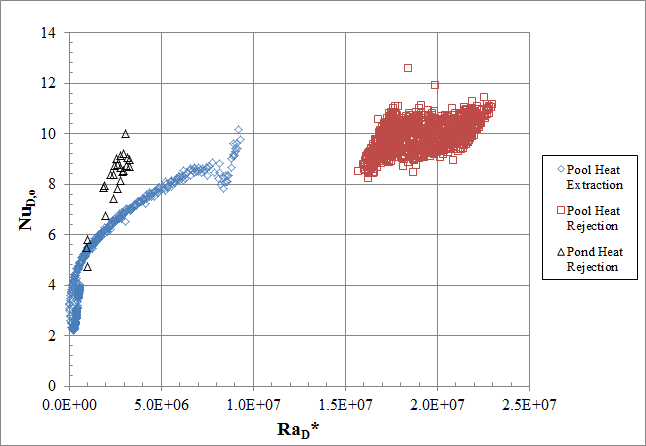
\includegraphics[width=0.8\textwidth]{PoolVsPond_075_2625H_15V.png}
		\caption[3/4 in.\ (19 mm) dia.\ 2.625 in.\ H x 1.3 in.\ V (67 mm x 33 mm) pool vs.\ pond comparison]{$\mbox{Nu}_{D,o}$ vs.\ $\mbox{Ra}_D^*$ plot of pond and pool heat extraction and rejection data for the 3/4 in.\ (19 mm) dia.\ HDPE pipe with 2.625 in.\ H x 1.3 in.\ V (67 mm x 33 mm) tube-tube spacing}
		\label{fig:ExpResult:FinalData:PoolVsPond_075_2625H_15V}
	\end{figure}
	
	\begin{figure}
		\centering
		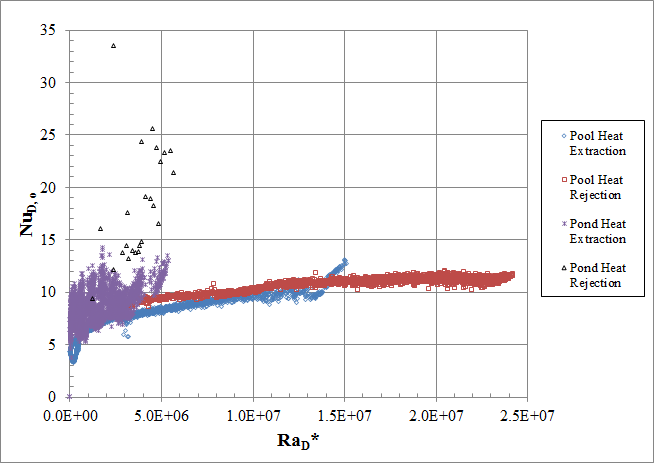
\includegraphics[width=0.8\textwidth]{PoolVsPond_075_2625H_2625V.png}
		\caption[3/4 in.\ (19 mm) dia.\ 2.625 in.\ H x 2.625 in.\ V (67 mm x 67 mm) pool vs.\ pond comparison]{$\mbox{Nu}_{D,o}$ vs.\ $\mbox{Ra}_D^*$ plot of pond and pool heat extraction and rejection data for the 3/4 in.\ (19 mm) dia.\ HDPE pipe with 2.625 in.\ H x 2.625 in.\ V (67 mm x 67 mm) tube-tube spacing}
		\label{fig:ExpResult:FinalData:PoolVsPond_075_2625H_2625V}
	\end{figure}

	\begin{figure}
		\centering
		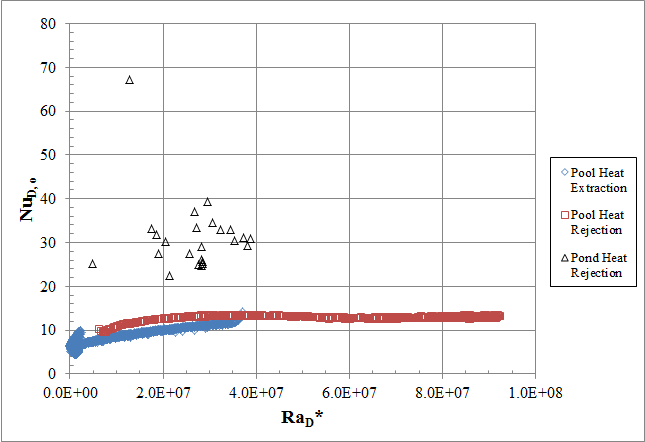
\includegraphics[width=0.8\textwidth]{PoolVsPond_125_4125H_2625V.png}
		\caption[1-1/4 in.\ (32 mm) dia.\ 4.125 in.\ H x 2.625 in.\ V (105 mm x 67 mm) pool vs.\ pond comparison]{$\mbox{Nu}_{D,o}$ vs.\ $\mbox{Ra}_D^*$ plot of pond and pool heat extraction and rejection data for the 1-1/4 in.\ (32 mm) dia.\ HDPE pipe with 4.125 in.\ H x 2.625 in.\ V (105 mm x 67 mm) tube-tube spacing}
		\label{fig:ExpResult:FinalData:PoolVsPond_125_4125H_2625V}
	\end{figure}

This suggests that there is something about the laboratory experimental apparatus that does not represent realistic operating conditions. In this context, \textit{realistic operating conditions} is defined as conditions under which we would expect actual SHWEs to operate. This would include being in a surface water body that is much deeper than the indoor test pool.

The pool is 15 ft (4.5 m) in diameter and is operating at water depth of 42 in.\ (1.1 m). Two of the coil configurations tested in the pool used 2.625 in.\ (67 mm) vertical tube-tube spacing. From Table \ref{tab:ExpMethod:HeatRej:Method:SWHEGeometry1} we can see that the nominal coil height is 14 in.\ (0.35 m) for these particular coil configurations. The coil was situated directly in the center of the pool in the lateral directions and was suspended approximately in the middle of the water column. Under these operating conditions, the coil is approximately 14 in.\ (0.35 m) above the pool bottom and 14 in.\ (0.35 m) below the water surface.

It is worth noting that all heat extraction data, along with the pool heat rejection data, were all collected with thermally enhanced HDPE. This thermally enhanced HDPE pipe has a thermal conductivity that is 75\% higher \citep{Gonthier2012} than standard PE3408 HDPE. In order to assess the potential differences introduced in outside Nusselt numbers due to the variations in pipe thermal conductivity, a simulation was set up to simulate heat exchanger performance, while fixing certain critical parameters.  The critical parameters which were fixed during the simulation are: SWHE (pipe) length, pipe diameters, SWHE diameters, SHWE configuration, circulating fluid flow rate, surface water temperature, heat pump load, and heat pump COP. The thermal conductivities for standard HDPE pipe, thermally enhanced HDPE, and copper were tested. 

The details of this simulation will be discussed in detail in Section \ref{sec:DesignTools:Derivation}, but briefly explained here. The simulation uses the outside SWHE convection correlations developed in Chapter \ref{ch:Correlation} to determine SWHE outside convection thermal resistance. Other calculations are similar to what was described in Section \ref{sec:ExpResult:HeatRej:DataAnalysis}.  The simulation is given a fixed inlet temperature, and from there it iteratively determines the required SWHE tube length to meet a fixed heat transfer rate. In order to fix the tube length, a range of inlet temperatures were given to the simulation and the results below were interpolated between data points to determine the desired information at the `fixed' tube length. Table \ref{tab:ExpResult:FinalData:FixedParams1} shows the thermal resistances and overall heat transfer coefficient from the simulation and Table \ref{tab:ExpResult:FinalData:FixedParams2} shows the temperatures calculated from the simulation.

\begin{table}[h]
	\centering
	\caption{Fixed parameter simulation results: thermal resistances and overall heat transfer coefficient}
	\label{tab:ExpResult:FinalData:FixedParams1}
	\begin{tabular}{r | c c c c c }
	\hline
	Tube & \multirow{2}{*}{$R_{conv,i}$} & \multirow{2}{*}{$R_{p,cond}$} & \multirow{2}{*}{$R_{conv,o}$} & \multirow{2}{*}{$UA_s$} \\
	Material & & & & \\
	\hline
	& $K/W$ & $K/W$ & $K/W$ & $W/K$  \\
	\hline\hline
	STD & $1.26 \cdot 10^{-4}$ & $1.63 \cdot 10^{-3}$ & $5.52 \cdot 10^{-4}$ & 434 \\
	\hline
	TEHDPE & $1.30 \cdot 10^{-4}$ & $9.73 \cdot 10^{-4}$ & $5.52 \cdot 10^{-4}$ &  605 \\
	\hline
	Cu & $1.38 \cdot 10^{-4}$ & $1.71 \cdot 10^{-6}$ & $5.54 \cdot 10^{-4}$ &  1447 \\
	\hline
	\end{tabular}
\end{table}

\begin{table}[h]
	\centering
	\caption{Fixed parameter simulation results: temperatures}
	\label{tab:ExpResult:FinalData:FixedParams2}
	\begin{tabular}{r | c c c | c c c c }
	\hline
	 Tube & \multirow{2}{*}{$T_{f,in}$} & \multirow{2}{*}{$T_{MFT}$} & \multirow{2}{*}{$T_{f,out}$} & \multirow{2}{*}{$T_{p,s,i}$} & \multirow{2}{*}{$T_{p,s,o}$} & \multirow{2}{*}{$T_{film,o}$} & Lake \\
	 Material & & & & & & & Temp \\
	\hline
	& $^\circ$C & $^\circ$C & $^\circ$C & $^\circ$C & $^\circ$C & $^\circ$C & $^\circ$C \\
	\hline\hline
	STD & 34.3 & 31.3 & 28.7 & 30.7 & 23.6 & 22.3 & 21.1 \\
	\hline
	TEHDPE & 31.5 & 28.4 & 25.9 & 27.8 & 23.6 & 22.3 & 21.1 \\
	\hline
	Cu & 27.8 & 24.2 & 22.2 & 23.6 & 23.6 & 22.3 & 21.1 \\
	\hline
	\end{tabular}
\end{table}

From Table \ref{tab:ExpResult:FinalData:FixedParams1}, we see that changing the pipe wall thermal conductivity has little to no affect on the inside thermal resistance. This is expected since flow rate and pipe inside diameter are fixed. The minor variations can be attributed to the changing fluid properties due to mean fluid temperature variations. Pipe conduction resistance variations are attributed entirely to the different thermal conductivities of the pipe materials. This is because diameters and pipe length were all fixed. 

Initially, outside convective resistance was expected to increase with increasing pipe thermal conductivity because all the temperatures, including pipe outside surface temperature, were expected to move closer to the surface water temperature. This would have resulted in a smaller temperature difference between the pipe outside surface and the lake temperatures, which would have resulted in a smaller outside film temperature and thus lower outside convection coefficient. However, this did not turn out to be the case. Table \ref{tab:ExpResult:FinalData:FixedParams2} shows the variations in entering, exiting, and mean fluid temperatures, as well as pipe surface temperatures. As expected, all temperatures did move closer to the surface water temperature, however, in this example, the outside film temperature did not change and therefore the driving potential for the outside convection remained constant. 

This result was not expected initially; however, if we perform a surface heat balance on the exterior surface of the SWHE and perform some analysis of the fundamental equations, we will see that the results are plausible. Equation \ref{eq:ExpResult:FinalData:SWHESurfHTBal} shows a surface heat balance for the SWHE exterior surface where the pipe conduction heat transfer is balanced by the outside convective heat transfer.

\begin{equation}
	\dot{Q}_{SWHE,p,cond} = \frac{T_{p,s,o} - T_{sw}}{R_{conv,o}}
	\label{eq:ExpResult:FinalData:SWHESurfHTBal}
\end{equation}

Examining Equation \ref{eq:ExpResult:FinalData:SWHESurfHTBal}, we will see that even by fixing heat transfer rate and surface water temperature, the pipe outside surface temperature and outside convective resistances are not known. However, we know that outside convective resistance is a function of Nusselt number, Nusselt number is a function of Rayleigh number, and Rayleigh number is a function of driving potential which is expressed as a temperature difference or a heat flux. This is shown in Equations \ref{eq:ExpResult:FinalData:Rout}, \ref{eq:ExpResult:FinalData:Ra}, and \ref{eq:ExpResult:FinalData:TempDiff}.

\begin{equation}
	R_{conv,o} = f(Nu_{D,o})
	\label{eq:ExpResult:FinalData:Rout}
\end{equation}

\begin{equation}
	Nu_{D,o} = f(Ra \, \mbox{or} \, Ra^*)
	\label{eq:ExpResult:FinalData:Ra}
\end{equation}

\begin{equation}
	Ra \, \mbox{or} \, Ra^* = f(T_{p,s,o}-T_{sw} \, \mbox{or} \, \dot{q})
	\label{eq:ExpResult:FinalData:TempDiff}
\end{equation}

Through careful examination we can see that driving potential, which is expressed as a temperature difference or a heat flux, is inversely proportional to outside convective resistance. Therefore, as driving potential increases outside convective resistance decreases. The reverse is also true. In our situation, because all other parameters, such as SWHE configuration, pipe diameter, surface water temperature, and heat transfer rate are all held constant, the driving potential and outside convective resistance must be the same if Equation \ref{eq:ExpResult:FinalData:SWHESurfHTBal} is to `balance'.

Therefore, we do not expect the outside convection coefficients to be affected by tube thermal conductivity. Thus, the variations shown above in Figures \ref{fig:ExpResult:FinalData:PoolVsPond_075_2625H_15V}, \ref{fig:ExpResult:FinalData:PoolVsPond_075_2625H_2625V}, and \ref{fig:ExpResult:FinalData:PoolVsPond_125_4125H_2625V} cannot be attributed to pipe material changes.

Another possible theory to explain the differences in outside Nusselt numbers shown above in Figures \ref{fig:ExpResult:FinalData:PoolVsPond_075_2625H_15V}, \ref{fig:ExpResult:FinalData:PoolVsPond_075_2625H_2625V}, and \ref{fig:ExpResult:FinalData:PoolVsPond_125_4125H_2625V} is the differences in free stream distances around the SWHE between the pond and the pool. \cite{Hansen2011} conducted a ``Lake Bottom Proximity" test where the affects of testing the SWHE suspended in the water column as is shown in Figure \ref{fig:ExpMethod:HeatRej:Apparatus:RejExpPond}, when compared to testing on the pond bottom were tested. For this test, the SWHE was allowed to reject heat under steady-state conditions while being suspended by the buoys in the pond. Once steady-state conditions were achieved, the SWHE was then lowered to the pond bottom and allowed to run again until steady state conditions were achieved.

From this experiment, \cite{Hansen2011} showed that the affects of the SWHE being on the pond bottom showed an increase in outside convection coefficient of around 8\%. He did, however, state that this result was within experimental uncertainty and that ``no definitive conclusion could be drawn from the test." This test was in heat rejection mode, therefore, the buoyant plume would be expected to flow upwards from the coil. Since the upper side of the coil was not subjected to a ``proximity test", nor was the coil constrained laterally, no conclusions can be drawn from his experiment.

I hypothesize that due to the fact that the depth of the pool is much less than the depth of the pond, the buoyant plume is constrained in either mode of operation. This may be the cause for the increased convective resistance in the pool when compared to experiments in the pond. We can also point out that in the pond the wind, sun, and precipitation will cause three dimensional mixing which will definitely not be uniform throughout the pond. There also may conceivably be affects from various varieties of aquatic vegetation and wildlife.

\section{Experimental Uncertainty}
\label{sec:ExpResult:Uncertainty}


\subsection{Measurement Uncertainty}
\label{subsec:ExpResult:Uncertainty:MeasuredUncerct}


Uncertainty in the inner and outer HDPE pipe diameters was determined by sampling 1 ft.\ (0.3 m) sections from each end of each coil tested. The inside and outside pipe diameters were then measured using telescoping gauges and a micrometer calibrated to 0.0001 in.\ (0.00254 mm), with the exception of the 1 in.\ pipe inside diameter; a telescoping gauge with the measurement range required to measure this inside diameter could not be located at the time the measurements were performed. The outside and inside diameter of each end of the 1 ft.\ (0.3 m) sections were measured at four different angles: 0-180$^\circ$, 90-270$^\circ$, 45-235$^\circ$, and 135-315$^\circ$. The four measurements were necessary to account for potential eccentricity in the pipe and to determine the average pipe diameter as is shown in Equation \ref{eq:ExpResult:Uncertainty:Dave}. 

\begin{equation}
	D_{sec} = \frac{D_{sec,1} + D_{sec,2} + D_{sec,3}+ D_{sec,4}}{4}
	\label{eq:ExpResult:Uncertainty:Dave}
\end{equation}

To determine the uncertainty in the pipe diameters, all of the average section diameters (Equation \ref{eq:ExpResult:Uncertainty:Dave}) for a give pipe size were taken and the standard deviation was determined as is shown in Equation \ref{eq:ExpResult:Uncertainty:STDEV} \citep{Taylor1997}.

\begin{equation}
	\sigma_{D} = \sqrt{\frac{1}{N_{D,sec}-1} \sum (D_{sec} - \bar{D})^2}
	\label{eq:ExpResult:Uncertainty:STDEV}
\end{equation}

For reference, Table \ref{tab:ExpResult:Uncertainty:ASTMPipe} shows the HDPE pipe dimensions as specified in \cite{ASTMD3035}. The average outside and inside pipe diameters as calculated from the standard can be seen in Table \ref{tab:ExpResult:Uncertainty:AveDia}. Incidentally, the average diameters shown in Table \ref{tab:ExpResult:Uncertainty:AveDia} are the dimensions listed in the HDPE manufacturer dimensional specification sheets.

\begin{table}[h]
	\centering
	\caption{Specified HDPE pipe dimensions from \cite{ASTMD3035}}
	\label{tab:ExpResult:Uncertainty:ASTMPipe}
	\begin{tabular}{p{2.5cm} | c c c c}
	\hline
	Nominal & \multirow{2}{*}{$D_o$} & $D_o$ & Min. Wall & Wall \\
	Size & & Tolerance & Thickness & Tolerance \\
	\hline	
	\multicolumn{5}{c}{in. (mm)} \\
	\hline\hline
	3/4 (19) & 1.050 (26.27) & $\pm 0.004$ (0.102) & 0.095 (2.41) & +0.02 (0.51) \\
	\hline
	1 (25) & 1.315 (33.40) & $\pm 0.004$ (0.102) & 0.120 (3.05) & +0.02 (0.51) \\
	\hline
	1-1/4 (32) & 1.660 (42.16) & $\pm 0.004$ (0.102) & 0.151 (3.84) & +0.02 (0.51) \\
	\hline
	\end{tabular}
\end{table}

\begin{table}[h]
	\centering
	\caption{Mean outside and inside pipe diameter for HDPE pipe from \cite{ASTMD3035}}
	\label{tab:ExpResult:Uncertainty:AveDia}
	\begin{tabular}{l | c c}
	\hline	
	Nominal Size & $D_{o,ave}$ & $D_{i,ave}$ \\
	\hline
	\multicolumn{3}{c}{in. (mm)} \\
	\hline\hline
	3/4 (19) & 1.050 (26.27) & 0.844 (21.44) \\
	\hline
	1 (25) & 1.315 (33.40) & 1.059 (26.89) \\
	\hline
	1-1/4 (32) & 1.660 (42.16) & 1.342 (34.09)\\
	\end{tabular}
\end{table}

Table \ref{tab:ExpResult:Uncertainty:AveDiaMeas} shows the average inside and outside pipe diameters, as well as the absolute percent error when compared to the average diameters shown in Table \ref{tab:ExpResult:Uncertainty:AveDia}. Because the average measured diameters for each pipe size are all less than 1\% different from the mean diameter as determined by \cite{ASTMD3035}, we can assume that the diameter measurements will all be normally distributed around the mean diameters indicated in Table \ref{tab:ExpResult:Uncertainty:AveDia}.

\begin{table}[h]
	\centering
	\caption{Mean measured inside and outside diameter and absolute percent error from \cite{ASTMD3035}}
	\label{tab:ExpResult:Uncertainty:AveDiaMeas}
	\begin{tabular}{l | c c | c c}
	\hline
	Nominal Size & $D_{o,ave}$ & $|\mbox{\% Error}|$ & $D_{i,ave}$ & $|\mbox{\% Error}|$ \\
	\hline
	\multicolumn{5}{c}{in. (mm)} \\
	\hline\hline
	3/4 (19) & 1.059 (26.92) & 0.88 & 0.848 (21.54) & 0.47 \\
	\hline
	1 (25) & 1.322 (33.58) & 0.52 & N/A & N/A \\
	\hline
	1-1/4 (32) & 1.666 (42.32) & 0.36 & 1.341 (34.06) & 0.07 \\
	\hline	
	\end{tabular}
\end{table}

Table \ref{tab:ExpResult:Uncertainty:STDEVs} shows the standard deviations of the measured pipe diameters. Because the two standard deviations will capture the 95\% of the values that are normally distributed about the measured mean, two times the standard deviation indicated in Table \ref{tab:ExpResult:Uncertainty:STDEVs} is taken as the pipe diameter uncertainty.

\begin{table}[h]
	\centering
	\caption{Standard deviations of measured pipe diameters}
	\label{tab:ExpResult:Uncertainty:STDEVs}
	\begin{tabular}{l | c c}
	\hline
	Nominal Size & $\sigma_{D,o}$ & $\sigma_{D,i}$ \\
	\hline
	\multicolumn{3}{c}{in. (mm)} \\
	\hline\hline
	3/4 (19) & 0.0017 (0.043) & 0.0024 (0.061) \\
	\hline
	1 (25) & 0.0007 (0.017) & N/A \\
	\hline
	1-1/4 (32) & 0.0028 (0.071) & 0.0046 (0.117) \\
	\hline	
	\end{tabular}
\end{table}

Temperature sensors were calibrated as described in Section \ref{subsec:ExpMethod:Instr:TempCal}. There, an example was given for which the correlated maximum absolute error was shown to be 0.11$^\circ$F (0.06$^\circ$C), which corresponds to a maximum absolute percent error of 0.13\%. As a conservative estimate, thermsitor uncertainty was taken to be 0.18$^\circ$F (0.1$^\circ$C).

Flow meters were calibrated as described in Section \ref{subsec:ExpMethod:Instr:FlowCal}. The ``Omega" flow meter was calibrated to a maximum absolute percent error within 0.6\%  and the ``Gem" flow meter was calibrated a maximum absolute percent error within 1.46\%. These values were taken as the calculated flow measurement uncertainty.

The uncertainty from each of the SWHE geometrical parameters are shown below in Table \ref{tab:ExpResult:Uncertainty:Parameters}. SWHE inside and outside diameters were determined by using a tape measure. Uncertainty from the inside and outside SWHE diameter measurements were given based on the authors judgment of the measurement accuracy. SWHE length was not measured by the author. Coils were ordered from the manufacture to be 500 ft.\ (152.4 m) in length and the SWHE length uncertainty is another estimate from the author of the uncertainty in SWHE length.

\begin{table}[h]
	\centering
	\caption{Experimental uncertainty for SWHE measured geometrical parameters}
	\label{tab:ExpResult:Uncertainty:Parameters}
	\begin{tabular}{l|l}
		\hline
		\multicolumn{2}{c}{Parameter Uncertainty} \\
		\hline\hline
		$w_{SWHE,D,o}$ & $\pm$ 1 in.\ (25 mm) \\
		\hline
		$w_{SWHE,D,i}$ & $\pm$ 1 in.\ (25 mm) \\
		\hline
		$w_{L}$ & $\pm$ 3.9 in.\ (0.1 m) \\
		\hline	
	\end{tabular}
\end{table}

\subsection{Uncertainty Analysis Methodology}
\label{subsec:ExpResult:Uncertainty:Method}

The uncertainty analysis was performed in order to quantify the uncertainty associated with the measured data. This uncertainty analysis gives an indication of the potential errors associated with the measured data and how the measurement uncertainty affects the analysis. It was also important in order to make an educated decision regarding which data points will yield the best correlation for outside convective resistance. From \cite{Hansen2011}, an upper limit of 70\% was used as the upper limit for outside Nusselt number uncertainty due to the large amount of scatter and uncertainty in the data. \cite{Hansen2011} performed an uncertainty analysis as is outlined in \cite{HolmanGajda1984} and shown in Equation \ref{eq:ExpResult:Uncertatiny:GeneralUncertainty}. Using this method, the uncertainty of the independent variables of a given parameter are summed together in quadrature to form the parameter's total uncertainty. This method assumes that all variables are independent from one another.

	\begin{equation}
		U_F = \sqrt{\left(\frac{\partial F}{\partial x_1} \, w_1 \right)^2 + \left(\frac{\partial F}{\partial x_2} \, w_2 \right)^2 + \cdots + \left(\frac{\partial F}{\partial x_n} \, w_n \right)^2}
		\label{eq:ExpResult:Uncertatiny:GeneralUncertainty}
	\end{equation}
	
After examining the uncertainty results from \cite{Hansen2011}, it was apparent that some steps could be taken to minimize the experimental uncertainty. This is because of the fact that some variables, which were treated as independent by \cite{Hansen2011}, were not truly independent. Also from \cite{Hansen2011}, the data was shown to have a high sensitivity to inside pipe diameter. In order to account for this, samples from HPDE pipes were taken and measured in order to estimate the uncertainty of the outside and inside diameters. This is in contrast to taking the uncertainty from \cite{ASTMD3035}, as was done in \cite{Hansen2011}.

The uncertainty analysis performed for this work was performed, generally, as was performed in \cite{Hansen2011} and outlined in \cite{HolmanGajda1984}, however, a few critical adjustments were made. These adjustments affect the way the heat transfer rate uncertainty and pipe thermal resistance uncertainty were calculated.

Generally when calculating a heat exchanger's heat transfer rate (Equations \ref{eq:ExpResult:HeatRej:DataAnalysis:HXHeatRate} and \ref{eq:ExpResult:HeatRej:DataAnalysis:HXMaxHeatRate}) we are not primarily concerned with absolute temperature measurement. We are, however, primarily concerned about the overall temperature difference between the heat exchanger inlet and outlet. If there is expected uncertainty in both the inlet and outlet temperature measurement, the relative proximity of the temperature measurements to one another can greatly affect the heat transfer uncertainty.

To illustrate this point, if the uncertainty of inlet and outlet temperature measurements is $\pm$ $0.18^\circ$F ($0.1^\circ$C), and the inlet and outlet temperatures were measured to be 66.2$^\circ$F (19.0$^\circ$C) and 68$^\circ$F (20.0$^\circ$C), respectively, then the heat transfer uncertainty would be expected to be quite high. Similarly, if the inlet and outlets were measured to be 50.0$^\circ$F (10.0$^\circ$C) and 86$^\circ$F (30.0$^\circ$C), respectively, then the heat transfer uncertainty would be expected to be quite low. 

To account for uncertainty in the heat transfer, Equation \ref{eq:ExpResult:Uncertatiny:GeneralUncertainty} was modified to account for this sensitivity to temperature difference as is shown in Equation \ref{eq:ExpResult:Uncertatiny:QUncertainty}.

	\begin{equation}
		U_{\dot{Q},SWHE} = \sqrt{\left(\frac{w_{\dot{m}}}{\dot{m}}\right)^2 + \left(\frac{w_{cp}}{c_p}\right)^2 + \left(\frac{\sqrt{w_{T,f,in}^2 + w_{T,f,out}^2}}{T_{f,in} - T_{f,out}}\right)^2}
		\label{eq:ExpResult:Uncertatiny:QUncertainty}
	\end{equation}
	
This formulation weights the uncertainty of the temperature difference, rather than simply the uncertainty of each temperature measurement independently. As the temperature difference becomes small, the weight of their uncertainty will have a larger effect than would occur if the temperature difference is quite large.

The only other instance where the uncertainty analysis deviates from what is shown in Equation \ref{eq:ExpResult:Uncertatiny:GeneralUncertainty} is when calculating the experimental uncertainty of the pipe conduction resistance (Equation \ref{eq:ExpResult:HeatRej:DataAnalysis:PipeResist}). This is shown below in Equation \ref{eq:ExpResult:Uncertatiny:RcUncertainty} where the $D_o/D_i$ is treated as one term.  

	\begin{equation}
		U_{R,cond} = \sqrt{e_{D_o/D_i}^2 + e_{kp}^2 + e_{L}^2}
		\label{eq:ExpResult:Uncertatiny:RcUncertainty}
	\end{equation}
	
	\centerline{where:}
	
	\begin{equation*}
	e_{D_o/D_i} = \frac{\partial \dot{R}_{cond}}{\partial (D_o/D_i)} \cdot w_{D_o/D_i}
	\end{equation*}
	
	\begin{equation*}
	e_{k_p} = \frac{\partial \dot{R}_{cond}}{\partial k_p} \cdot w_{kp}
	\end{equation*}

	\begin{equation*}
	e_{L} = \frac{\partial\dot{R}_{cond}}{\partial L} \cdot w_{L}
	\end{equation*}
	
The reason for this is because the outside and inside pipe diameters are expected to vary together. This could occur due to pipe pressure or temperature changes which could cause the pipe to expand or contract. 

 All SWHEs tested used HDPE tubing with the same diameter ratio, which is the ratio of pipe outside diameter to pipe wall thickness, as is shown in Equation \ref{eq:ExpResult:Uncertainty:SDR}. From this equation, it can be shown that the ratio of outside pipe diameter to inside pipe diameter is constant for all pipes with the same diameter ratio. This expression is shown in Equation \ref{eq:ExpResult:Uncertainty:DoDi}

\begin{equation}
	SDR = \frac{D_o}{t}
	\label{eq:ExpResult:Uncertainty:SDR}
\end{equation}

\begin{equation}
	\frac{D_o}{D_i} = \left(1 - \frac{2}{SDR} \right)^{-1}
	\label{eq:ExpResult:Uncertainty:DoDi}
\end{equation}

Due to the fact that the measured diameters are expected to be normally distributed about the average diameter as was shown previously, two times the standard deviation of the measured outside diameter to inside diameter can be used and the uncertainty for $D_o/D_i$, $w_{D_o/D_i}$. Also, because all pipe sizes are expected to have the same ratio of outside to inside diameter, the analysis can be simplified to only use one value of $w_{D_o/D_i}$ for all pipe sizes. From the measured pipe diameters, the standard deviation for all ratios of measured outside to inside pipe diameter was determined to be 0.0048 in.\ (0.123 mm).

The experimental uncertainty for each series of tests is broken down in the following sections by applying the previously described methods.

\subsection{Pond Heat Rejection Data Uncertainty}
\label{subsec:ExpResult:Uncertainty:PondRej}

In Figure \ref{fig:ExpResult:Uncertainty:PondHeatRej:Histogram} we can see a histogram of the experimental outside Nusselt number uncertainty from the data collected in the pond during the heat rejection experiments. Experimental uncertainty is lower when compare to the experimental uncertainty from \cite{Hansen2011}. This is attributed to tighter uncertainties on pipe diameters, as well as the improved methods for determining heat transfer rate uncertainty and pipe conduction resistance uncertainty as was explained in Section \ref{subsec:ExpResult:Uncertainty:Method}.

\begin{figure}
	\centering
	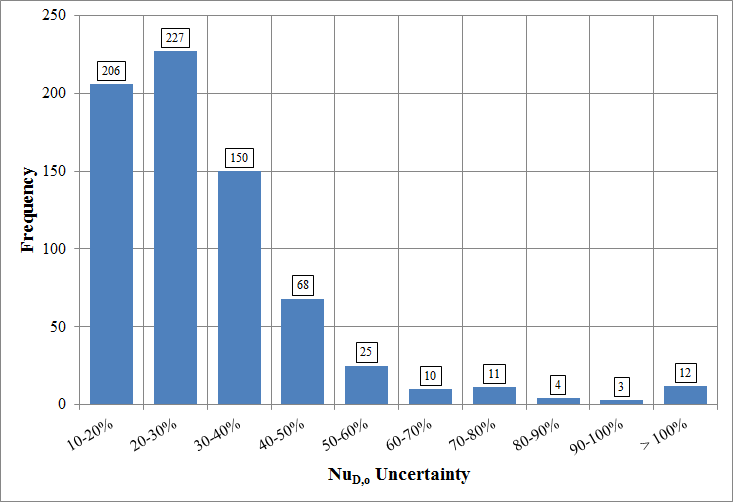
\includegraphics[width=0.8\textwidth]{HistogramPondHeatRej.png}
	\caption{Pond heat rejection data outside Nusselt number uncertainty histogram}
	\label{fig:ExpResult:Uncertainty:PondHeatRej:Histogram}
\end{figure}

In Figure \ref{fig:ExpResult:Uncertainty:PondHeatRej:HTUncertainty}, we can see that the heat transfer uncertainty drops with increasing heat transfer rate. This occurs as expected due to the way heat transfer uncertainty is calculated. 

\begin{figure}
	\centering
	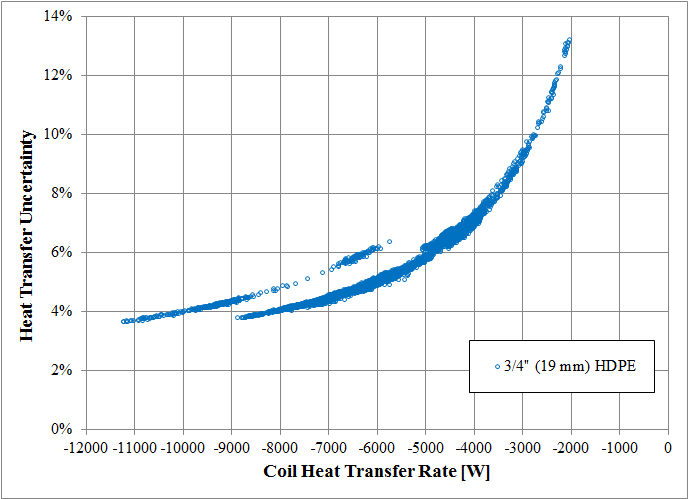
\includegraphics[width=0.8\textwidth]{HTUncertaintyVsHTRatePondHeatRej.png}
	\caption{Pond heat rejection data heat transfer uncertainty vs.\ SWHE heat transfer rate}
	\label{fig:ExpResult:Uncertainty:PondHeatRej:HTUncertainty}
\end{figure}

Another point that can be clearly seen in Figure \ref{fig:ExpResult:Uncertainty:PondHeatRej:HTUncertainty} is the distinction between the discrete tube sizes. This is directly due to the increase in flow rate between the tube sizes. This effect is due to the smaller temperature difference across the SWHE which necessarily must occur if flow rate is increased and heat transfer rate is held constant.

Given that this data was collected outdoors in an open pond, the estimated heat transfer uncertainty appears to be reasonably good. This is primarily due to the fact that flow meters and temperature sensors were tightly calibrated. Great care was taken to preserve these calibrations, as this was one of the few parameters that could be controlled when experimenting in a highly variable environment.

In Figure \ref{fig:ExpResult:Uncertainty:PondHeatRej:QCoilNuUncertainty}, we can see the outside Nusselt number uncertainty plotted against the heat transfer rate. Here, we also see decreasing Nusselt number uncertainty with increasing heat transfer rate. Also visible to a small degree is the distinction between different tube sizes. There is also a large degree of scatter visible in the plot. Even though flow and temperature sensors were tightly calibrated, and numerous other steps were taken to tighten the experimental uncertainty, we cannot get away from the fact that this data was collected in an uncontrolled environment. The scatter that is seen in the plot is largely due to the parameters which were out of our control. A few examples of these parameters are: wind, ambient temperature, underwater currents and eddies, aquatic wildlife, etc.

\begin{figure}
	\centering
	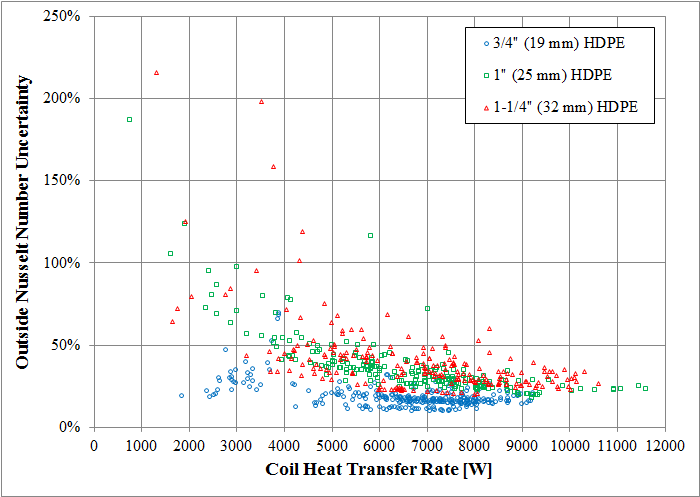
\includegraphics[width=0.8\textwidth]{QCoilNuUncertaintyPondHeatRej.png}
	\caption{Outside Nusselt number uncertainty vs.\ coil heat transfer rate}
	\label{fig:ExpResult:Uncertainty:PondHeatRej:QCoilNuUncertainty}
\end{figure}

\subsection{Pond Heat Extraction Data Uncertainty}
\label{subsec:ExpResult:Uncertainty:PondExtr}

Figure \ref{fig:ExpResult:Uncertainty:PondHeatExtr:HistogramPondHeatExtr} shows a histogram plot of the Nusselt number uncertainty for the pond heat extraction data. From this we can see that the pond heat extraction data has Nusselt number uncertainty values that are similar to the majority of the data taken in the pond during the heat rejection experiments. Again, this is an indication of the variability in the environment when testing in realistic operating conditions.

Heat transfer uncertainty is plotted against heat transfer rate in Figure \ref{fig:ExpResult:Uncertainty:PondHeatExtr:HTUncertaintyVsHTRatePondHeatExtr}. Here, again we see that the heat transfer uncertainty is quite good at high heat transfer rates. Outside Nusselt number uncertainty is plotted against heat transfer rate can be seen in Figure \ref{fig:ExpResult:Uncertainty:PondHeatExtr:QCoilNuUncertaintyUnfilteredPondHeatExtr}. The scatter in the data is due to the highly uncontrolled nature of the environment in which the data was collected.

 \begin{figure}
	\centering
	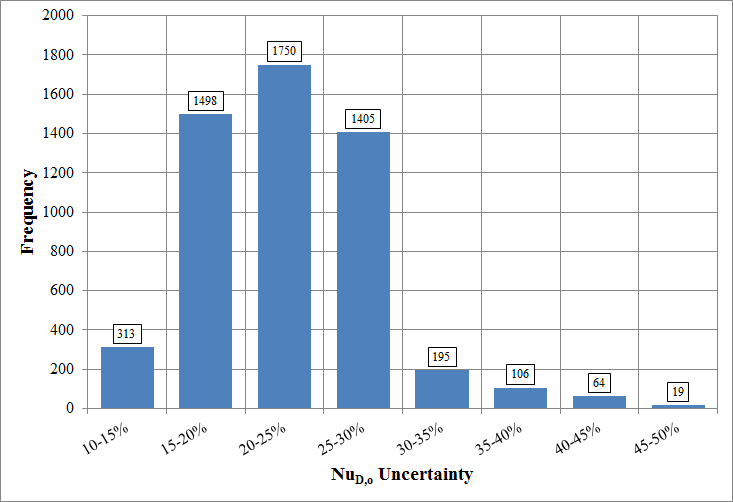
\includegraphics[width=0.8\textwidth]{HistogramPondHeatExtr.png}
	\caption{Pond heat extraction data Nusselt number uncertainty histogram}
	\label{fig:ExpResult:Uncertainty:PondHeatExtr:HistogramPondHeatExtr}
\end{figure}

\begin{figure}
	\centering
	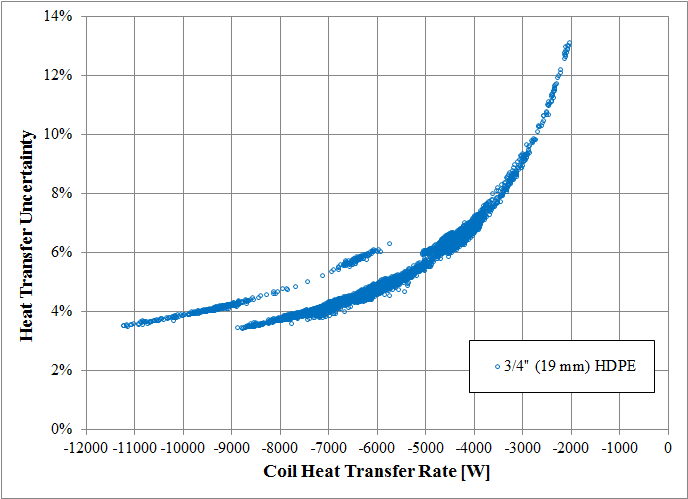
\includegraphics[width=0.8\textwidth]{HTUncertaintyVsHTRatePondHeatExtr.png}
	\caption{SWHE heat transfer uncertainty vs.\ SWHE heat transfer rate}
	\label{fig:ExpResult:Uncertainty:PondHeatExtr:HTUncertaintyVsHTRatePondHeatExtr}
\end{figure}

\begin{figure}
	\centering
	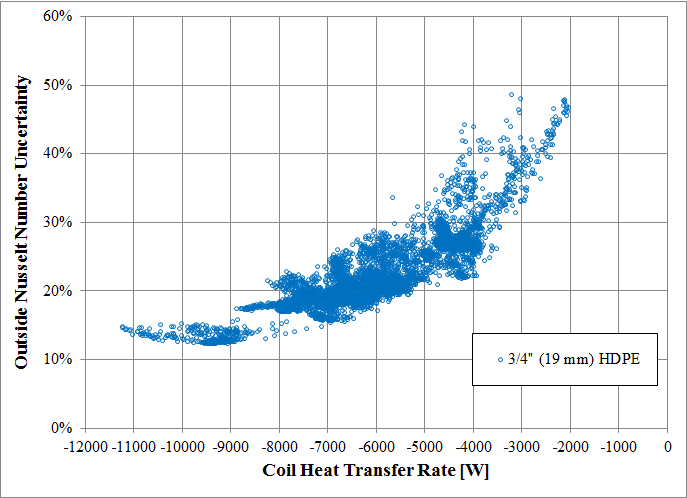
\includegraphics[width=0.8\textwidth]{QCoilNuUncertaintyUnfilteredPondHeatExtr.png}
	\caption{Pond heat extraction data outside Nusselt number uncertainty vs.\ coil heat transfer rate}	\label{fig:ExpResult:Uncertainty:PondHeatExtr:QCoilNuUncertaintyUnfilteredPondHeatExtr}
\end{figure}

\subsection{Pool Heat Rejection Data Uncertainty}
\label{subsec:ExpResult:Uncertainty:PoolRej}

In Figure \ref{fig:ExpResult:Uncertainty:PoolHeatRej:HistogramPoolHeatRej} we can see a histogram plot of the outside Nusselt number uncertainty for the pool heat rejection data. Nusselt number uncertainty is shown to be less than the uncertainty in the pond heat rejection data. This relates back to the fact that experiments performed in the pool had conditions which were more tightly controlled. In the pool, the pool water was not exposed to wind or other environmental conditions as occurred in the pond.

\begin{figure}
	\centering
	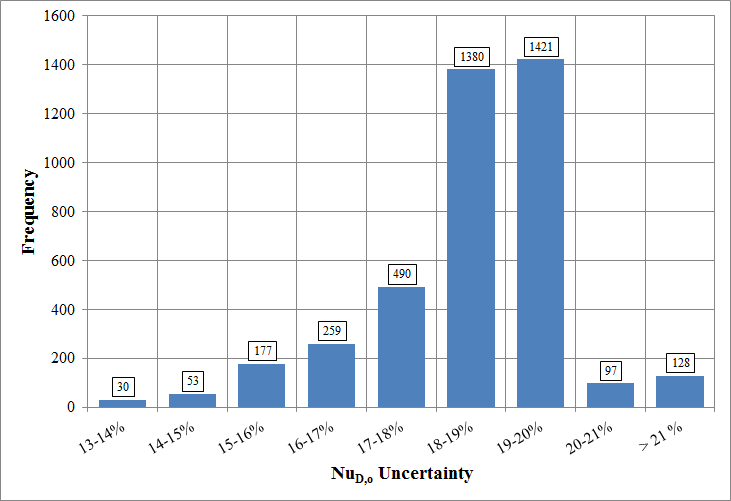
\includegraphics[width=0.8\textwidth]{HistogramPoolHeatRej.png}
	\caption{Pool heat rejection data Nusselt number uncertainty histogram}
	\label{fig:ExpResult:Uncertainty:PoolHeatRej:HistogramPoolHeatRej}
\end{figure}

Figure \ref{fig:ExpResult:Uncertainty:PoolHeatRej:QCoilHTUncertainty}, we can see the heat transfer uncertainty is quite low over the entire range of test data. The heat pumps used to perform heat rejection tests were not variable speed machines and any heat transfer variations seen are a direct result of machine performance varying over the course of the test. Here again the larger tube size is shown to have a higher heat transfer uncertainty, which is due to the changing flow rates between the two tube sizes.

\begin{figure}
	\centering
	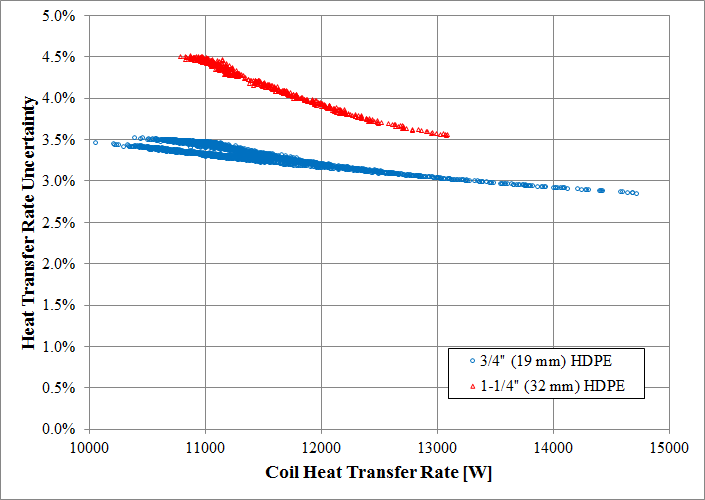
\includegraphics[width=0.8\textwidth]{QCoilHTUncertaintyPoolHeatRej.png}
	\caption{Pool heat rejection data heat transfer uncertainty vs.\ SWHE heat transfer rate}
	\label{fig:ExpResult:Uncertainty:PoolHeatRej:QCoilHTUncertainty}
\end{figure}

In Figure \ref{fig:ExpResult:Uncertainty:PoolHeatRej:QCoilNuUncertaintyUnfilteredPoolHeatRej} we can see the outside Nusselt number uncertainty plotted against SWHE heat transfer rate. Some scatter is visible in the data, but the outside Nusselt number uncertainty is significantly less than the outside Nusselt number uncertainty of the pond heat rejection data. 

\begin{figure}
	\centering
	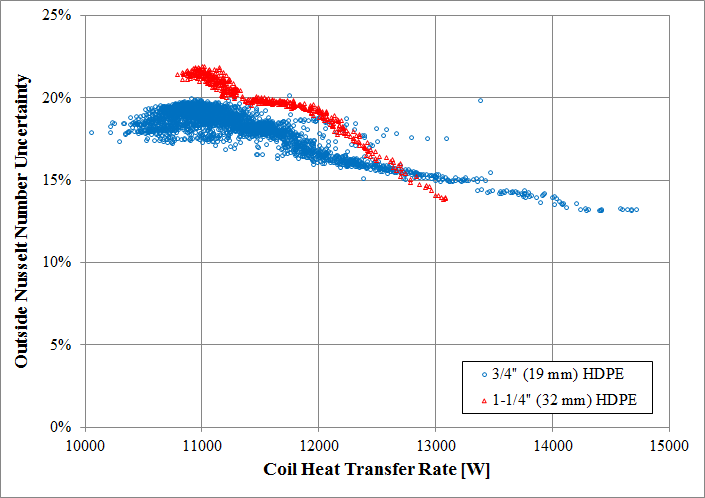
\includegraphics[width=0.8\textwidth]{QCoilNuUncertaintyUnfilteredPoolHeatRej.png}
	\caption{Pool heat rejection data outside Nusselt number uncertainty vs.\ SWHE heat transfer rate}	\label{fig:ExpResult:Uncertainty:PoolHeatRej:QCoilNuUncertaintyUnfilteredPoolHeatRej}
\end{figure}


\subsection{Pool Heat Extraction Data Uncertainty}
\label{subsec:ExpResult:Uncertainty:PoolExtr}

Figure \ref{fig:ExpResult:Uncertainty:PoolHeatExtr:HistogramPoolHeatExtr} shows a histogram plot of the outside Nusselt number uncertainty for the pool heat extraction data. In Outside Nusselt number uncertainty is similar to the previous data sets. Figure \ref{fig:ExpResult:Uncertainty:PoolHeatExtr:QCoilHTUncertainty}, we see the heat transfer uncertainty plotted against the heat transfer rate. This again is similar to the results presented previously.

\begin{figure}
	\centering
	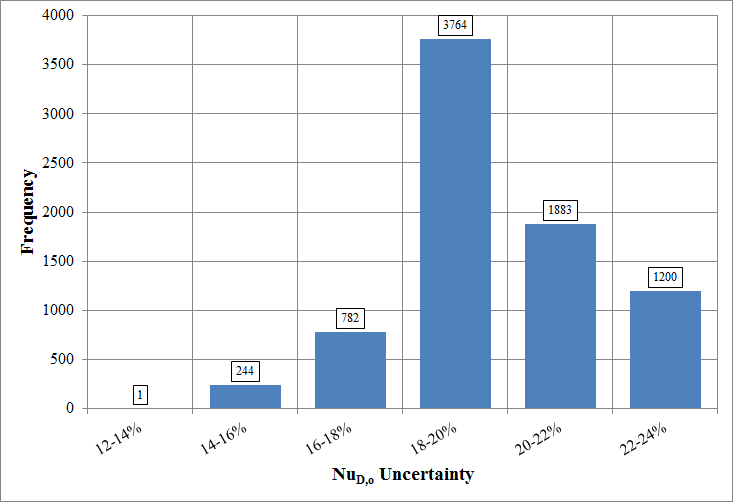
\includegraphics[width=0.8\textwidth]{HistogramPoolHeatExtr.png}
	\caption{Pool heat extraction data Nusselt number uncertainty histogram}
	\label{fig:ExpResult:Uncertainty:PoolHeatExtr:HistogramPoolHeatExtr}
\end{figure}

\begin{figure}
	\centering
	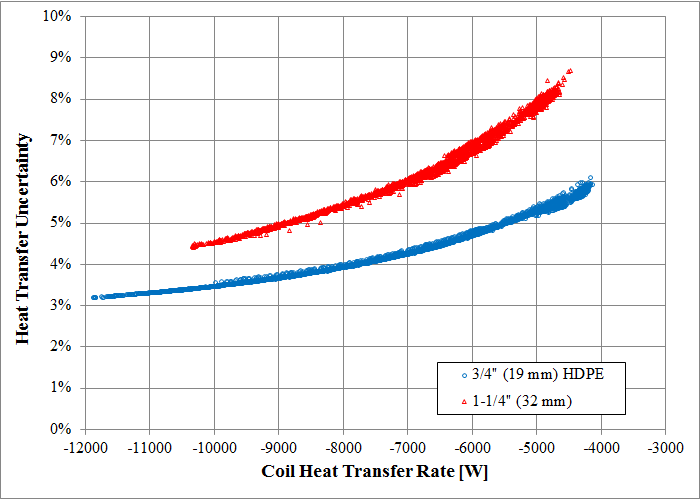
\includegraphics[width=0.8\textwidth]{QCoilHTUncertaintyPoolHeatExtr.png}
	\caption{Heat transfer uncertainty vs.\ heat transfer rate for the pool heat extraction data}
	\label{fig:ExpResult:Uncertainty:PoolHeatExtr:QCoilHTUncertainty}
\end{figure}

Figure \ref{fig:ExpResult:Uncertainty:PoolHeatExtr:QCoilNuUncertaintyUnfilteredPoolHeatExtr} shows the outside Nusselt number uncertainty plotted against heat transfer rate. It is worth noting that for these tests, circulating fluid flow rate dropped by about 18\% for the 1-1/4 in.\ (32 mm) test, and about 27\% for the 3/4 in.\ (19 mm) tests. This was due entirely to the viscosity of the circulating fluid increasing as the circulation fluid cooled. Additionally, the heat transfer rate dropped due entirely to the performance degradation of the heat pumps when operating at colder temperatures.

\begin{figure}
	\centering
	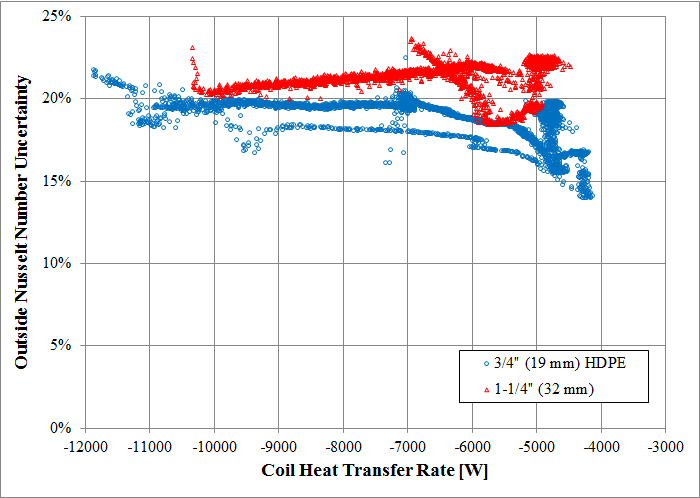
\includegraphics[width=0.8\textwidth]{QCoilNuUncertaintyUnfilteredPoolHeatExtr.png}
	\caption{Outside Nusselt Number Uncertainty Plotted Against Coil Heat Transfer Rate for the Pool Heat extraction Data}	\label{fig:ExpResult:Uncertainty:PoolHeatExtr:QCoilNuUncertaintyUnfilteredPoolHeatExtr}
\end{figure}
